\chapter{Computation and Representation}\label{chaprepres}

\begin{objectives} \label[objectives]{Distinguish-between-speci}

\begin{itemize}
\tightlist
\item
  Distinguish between \emph{specification} and \emph{implementation}, or
  equivalently between \emph{mathematical functions} and
  \emph{algorithms/programs}.
\item
  Representing an object as a string (often of zeroes and ones).
\item
  Examples of representations for common objects such as numbers,
  vectors, lists, graphs.
\item
  Prefix-free representations.
\item
  Cantor's Theorem: The real numbers cannot be represented exactly as
  finite strings.
\end{itemize}

\end{objectives}

\begin{quote}
\emph{``The alphabet (sic) was a great invention, which enabled men
(sic) to store and to learn with little effort what others had learned
the hard way -- that is, to learn from books rather than from direct,
possibly painful, contact with the real world.''}, B.F. Skinner
\end{quote}

\begin{quote}
\emph{``The name of the song is called `HADDOCK'S EYES.'''} {[}said the
Knight{]}

\emph{``Oh, that's the name of the song, is it?''} Alice said, trying to
feel interested.

\emph{``No, you don't understand,''} the Knight said, looking a little
vexed. \emph{``That's what the name is CALLED. The name really is `THE
AGED AGED MAN.'''}

\emph{``Then I ought to have said `That's what the SONG is called'?''}
Alice corrected herself.

\emph{``No, you oughtn't: that's quite another thing! The SONG is called
`WAYS AND MEANS': but that's only what it's CALLED, you know!''}

\emph{``Well, what IS the song, then?''} said Alice, who was by this
time completely bewildered.

\emph{``I was coming to that,''} the Knight said. \emph{``The song
really IS `A-SITTING ON A GATE': and the tune's my own invention.''}

Lewis Carroll, \emph{Through the Looking-Glass}
\end{quote}

To a first approximation, \emph{computation} is a process that maps an
\emph{input} to an \emph{output}.


\begin{marginfigure}
\centering
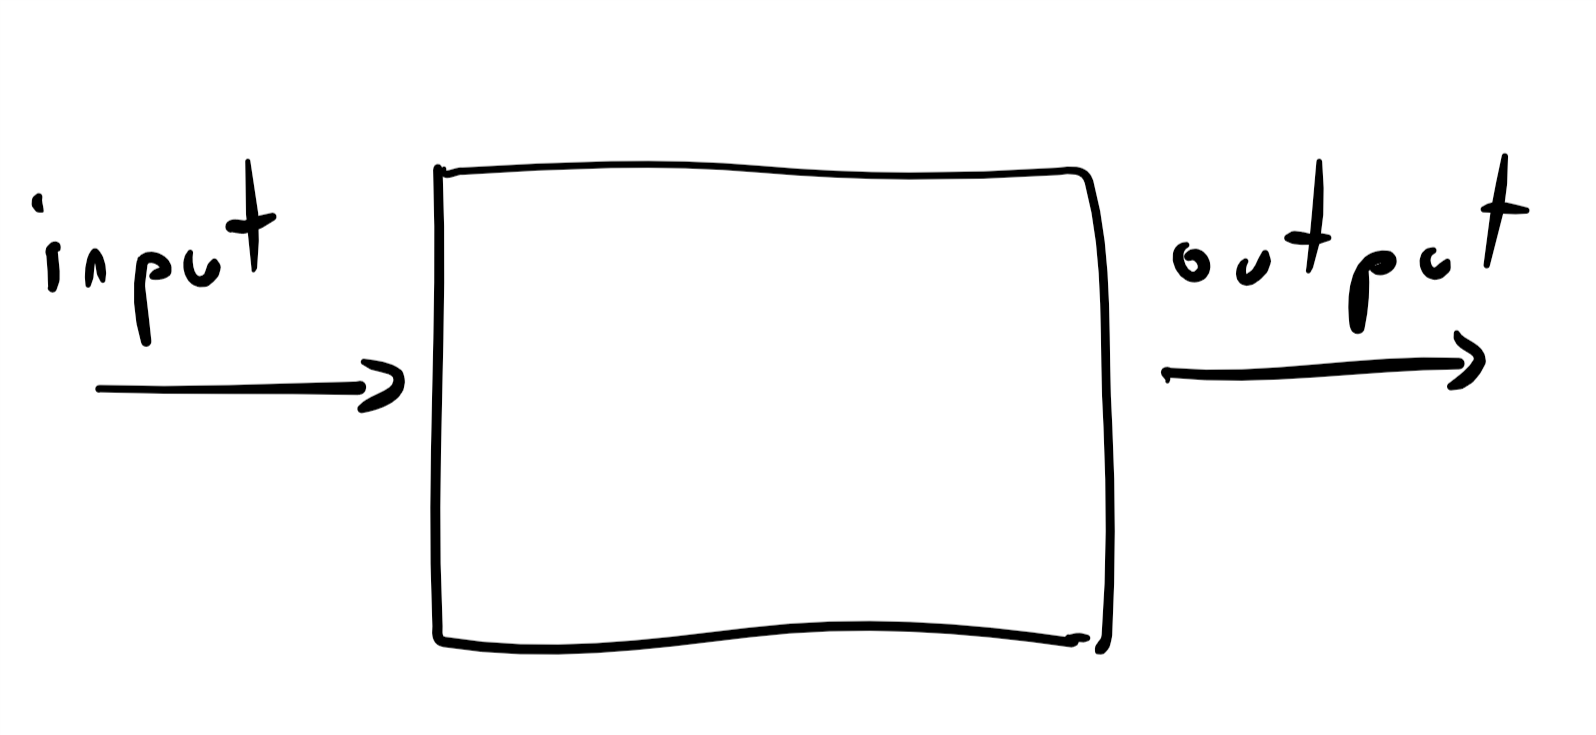
\includegraphics[width=\linewidth, height=1.5in, keepaspectratio]{../figure/input_output.png}
\caption{Our basic notion of \emph{computation} is some process that
maps an input to an output}
\label{computationinputtooutputfig}
\end{marginfigure}

When discussing computation, it is essential to separate the question of
\textbf{what} is the task we need to perform (i.e., the
\emph{specification}) from the question of \textbf{how} we achieve this
task (i.e., the \emph{implementation}). For example, as we've seen,
there is more than one way to achieve the computational task of
computing the product of two integers.

In this chapter we focus on the \textbf{what} part, namely defining
computational tasks. For starters, we need to define the inputs and
outputs. Capturing all the potential inputs and outputs that we might
ever want to compute on seems challenging, since computation today is
applied to a wide variety of objects. We do not compute merely on
numbers, but also on texts, images, videos, connection graphs of social
networks, MRI scans, gene data, and even other programs. We will
represent all these objects as \textbf{strings of zeroes and ones}, that
is objects such as \(0011101\) or \(1011\) or any other finite list of
\(1\)'s and \(0\)'s. (This choice is for convenience: there is nothing
``holy'' about zeroes and ones, and we could have used any other finite
collection of symbols.)


\begin{marginfigure}
\centering
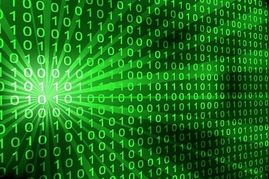
\includegraphics[width=\linewidth, height=1.5in, keepaspectratio]{../figure/zeroes-ones.jpg}
\caption{We represent numbers, texts, images, networks and many other
objects using strings of zeroes and ones. Writing the zeroes and ones
themselves in green font over a black background is optional.}
\label{zerosandonesgreenfig}
\end{marginfigure}

Today, we are so used to the notion of digital representation that we
are not surprised by the existence of such an encoding. But it is
actually a deep insight with significant implications. Many animals can
convey a particular fear or desire, but what is unique about humans is
\emph{language}: we use a finite collection of basic symbols to describe
a potentially unlimited range of experiences. Language allows
transmission of information over both time and space and enables
societies that span a great many people and accumulate a body of shared
knowledge over time.

Over the last several decades, we have seen a revolution in what we can
represent and convey in digital form. We can capture experiences with
almost perfect fidelity, and disseminate it essentially instantaneously
to an unlimited audience. Moreover, once information is in digital form,
we can \emph{compute} over it, and gain insights from data that were not
accessible in prior times. At the heart of this revolution is the simple
but profound observation that we can represent an unbounded variety of
objects using a finite set of symbols (and in fact using only the two
symbols \texttt{0} and \texttt{1}).

In later chapters, we will typically take such representations for
granted, and hence use expressions such as ``program \(P\) takes \(x\)
as input'' when \(x\) might be a number, a vector, a graph, or any other
object, when we really mean that \(P\) takes as input the
\emph{representation} of \(x\) as a binary string. However, in this
chapter we will dwell a bit more on how we can construct such
representations.

\section{Defining representations}\label{Defining-representations}

Every time we store numbers, images, sounds, databases, or other objects
on a computer, what we actually store in the computer's memory is the
\emph{representation} of these objects. Moreover, the idea of
representation is not restricted to digital computers. When we write
down text or make a drawing we are \emph{representing} ideas or
experiences as sequences of symbols (which might as well be strings of
zeroes and ones). Even our brain does not store the actual sensory
inputs we experience, but rather only a \emph{representation} of them.

To use objects such as numbers, images, graphs, or others as inputs for
computation, we need to define precisely how to represent these objects
as binary strings. A \emph{representation scheme} is a way to map an
object \(x\) to a binary string \(E(x) \in \{0,1\}^*\). For example, a
representation scheme for natural numbers is a function
\(E:\N \rightarrow \{0,1\}^*\). Of course, we cannot merely represent
all numbers as the string ``\(0011\)'' (for example). A minimal
requirement is that if two numbers \(x\) and \(x'\) are different then
they would be represented by different strings. Another way to say this
is that we require the encoding function \(E\) to be \emph{one to one}.

\subsection{Representing natural
numbers}\label{Representing-natural-numb}

We now show how we can represent natural numbers as binary strings. Over
the years people have represented numbers in a variety of ways,
including Roman numerals, tally marks, our own Hindu-Arabic decimal
system, and many others. We can use any one of those as well as many
others to represent a number as a string (see \cref{bitmapdigitsfig}).
However, for the sake of concreteness, we use the \emph{binary basis} as
our default representation of natural numbers as strings. For example,
we represent the number six as the string \(110\) since
\(1\cdot 2^{2} + 1 \cdot 2^1 + 0 \cdot 2^0 = 6\), and similarly we
represent the number thirty-five as the string \(y = 100011\) which
satisfies \(\sum_{i=0}^5 y_i \cdot 2^{|y|-i-1} = 35\). Some more
examples are given in the table below.


\begin{marginfigure}
\centering
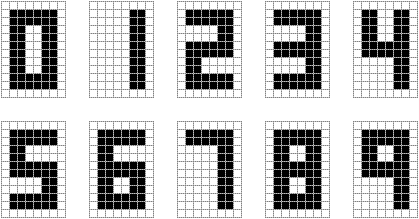
\includegraphics[width=\linewidth, height=1.5in, keepaspectratio]{../figure/digitsbitmap.png}
\caption{Representing each one the digits \(0,1,2,\ldots,9\) as a
\(12\times 8\) bitmap image, which can be thought of as a string in
\(\{0,1\}^{96}\). Using this scheme we can represent a natural number
\(x\) of \(n\) decimal digits as a string in \(\{0,1\}^{96n}\). Image
taken from
\href{http://blog.andersen.im/2010/12/autonomous-neural-development-and-pruning/}{blog
post of A. C. Andersen}.}
\label{bitmapdigitsfig}
\end{marginfigure}

\begin{longtable}[]{@{}ll@{}}
\caption{Representing numbers in the binary basis. The lefthand column
contains representations of natural numbers in the decimal basis, while
the righthand column contains representations of the same numbers in the
binary basis.}\tabularnewline
\toprule
\textbf{Number (decimal representation)} & \textbf{Number (binary
representation)}\tabularnewline
\midrule
\endfirsthead
\toprule
\textbf{Number (decimal representation)} & \textbf{Number (binary
representation)}\tabularnewline
\midrule
\endhead
0 & 0\tabularnewline
1 & 1\tabularnewline
2 & 10\tabularnewline
5 & 101\tabularnewline
16 & 10000\tabularnewline
40 & 101000\tabularnewline
53 & 110101\tabularnewline
389 & 110000101\tabularnewline
3750 & 111010100110\tabularnewline
\bottomrule
\end{longtable}

If \(n\) is even, then the least significant digit of \(n\)'s binary
representation is \(0\), while if \(n\) is odd then this digit equals
\(1\). Just like the number \(\floor{n/10}\) corresponds to ``chopping
off'' the least significant decimal digit (e.g.,
\(\floor{457/10}=\floor{45.7}=45\)), the number \(\floor{n/2}\)
corresponds to the ``chopping off'' the least significant \emph{binary}
digit. Hence the binary representation can be formally defined as the
following function \(NtS:\N \rightarrow \{0,1\}^*\) (\(NtS\) stands for
``natural numbers to strings''):

\[NtS(n) = \begin{cases}
            0    &  n=0 \\
            1    &  n=1 \\
            NtS(\floor{n/2}) parity(n) & n>1
\end{cases} \label{ntseq}\] where \(parity:\N \rightarrow \{0,1\}\) is
the function defined as \(parity(n)=0\) if \(n\) is even and
\(parity(n)=1\) if \(n\) is odd, and as usual, for strings
\(x,y \in \{0,1\}^*\), \(xy\) denotes the concatenation of \(x\) and
\(y\). The function \(NtS\) is defined \emph{recursively}: for every
\(n>0\) we define \(rep(n)\) in terms of the representation of the
smaller number \(\floor{n/2}\). It is also possible to define \(NtS\)
non-recursively, see \cref{binaryrepex}.

Throughout most of this book, the particular choices of representation
of numbers as binary strings would not matter much: we just need to know
that such a representation exists. In fact, for many of our purposes we
can even use the simpler representation of mapping a natural number
\(n\) to the length-\(n\) all-zero string \(0^n\).

\hypertarget{pythonbinary}{}
\begin{remark}[Binary representation in python (optional)] \label[remark]{pythonbinary}

We can implement the binary representation in \emph{Python} as follows:

\begin{code}
def NtS(n):# natural numbers to strings
    if n > 1:
        return NtS(n // 2) + str(n % 2)
    else:
        return str(n % 2)

print(NtS(236))
# 11101100

print(NtS(19))
# 10011
\end{code}

We can also use Python to implement the inverse transformation, mapping
a string back to the natural number it represents.

\begin{code}
def StN(x):# String to number
    k = len(x)-1
    return sum(int(x[i])*(2**(k-i)) for i in range(k+1))

print(StN(NtS(236)))
# 236
\end{code}

\end{remark}

\hypertarget{programmingrem}{}
\begin{remark}[Programming examples] \label[remark]{programmingrem}

In this book, we sometimes use \emph{code examples} as in
\cref{pythonbinary}. The point is always to emphasize that certain
computations can be achieved concretely, rather than illustrating the
features of Python or any other programming language. Indeed, one of the
messages of this book is that all programming languages are in a certain
precise sense \emph{equivalent} to one another, and hence we could have
just as well used JavaScript, C, COBOL, Visual Basic or even
\href{https://goo.gl/LKKNFK}{BrainF*ck}. This book is \emph{not} about
programming, and it is absolutely OK if you are not familiar with Python
or do not follow code examples such as those in \cref{pythonbinary}.

\end{remark}

\subsection{Meaning of representations
(discussion)}\label{Meaning-of-representation}

It is natural for us to think of \(236\) as the ``actual'' number, and
of \(11101100\) as ``merely'' its representation. However, for most
Europeans in the middle ages \texttt{CCXXXVI} would be the ``actual''
number and \(236\) (if they have even heard about it) would be the weird
Hindu-Arabic positional representation.\footnote{While the Babylonians
  already invented a positional system much earlier, the decimal
  positional system we use today was invented by Indian mathematicians
  around the third century. Arab mathematicians took it up in the 8th
  century. It first received significant attention in Europe with the
  publication of the 1202 book \emph{``Liber Abaci''} by Leonardo of
  Pisa, also known as Fibonacci, but it did not displace Roman numerals
  in common usage until the 15th century.} When our AI robot overlords
materialize, they will probably think of \(11101100\) as the ``actual''
number and of \(236\) as ``merely'' a representation that they need to
use when they give commands to humans.

So what is the ``actual'' number? This is a question that philosophers
of mathematics have pondered over throughout history. Plato argued that
mathematical objects exist in some ideal sphere of existence (that to a
certain extent is more ``real'' than the world we perceive via our
senses, as this latter world is merely the shadow of this ideal sphere).
In Plato's vision, the symbols \(236\) are merely notation for some
ideal object, that, in homage to the \href{https://goo.gl/b93h83}{late
musician}, we can refer to as ``the number commonly represented by
\(236\)''.

The Austrian philosopher Ludwig Wittgenstein, on the other hand, argued
that mathematical objects do not exist at all, and the only things that
exist are the actual marks on paper that make up \(236\), \(11101100\)
or \texttt{CCXXXVI}. In Wittgenstein's view, mathematics is merely about
formal manipulation of symbols that do not have any inherent meaning.
You can think of the ``actual'' number as (somewhat recursively) ``that
thing which is common to \(236\), \(11101100\) and \texttt{CCXXXVI} and
all other past and future representations that are meant to capture the
same object''.

While reading this book, you are free to choose your own philosophy of
mathematics, as long as you maintain the distinction between the
mathematical objects themselves and the various particular choices of
representing them, whether as splotches of ink, pixels on a screen,
zeroes and one, or any other form.

\section{Representations beyond natural
numbers}\label{Representations-beyond-na}

We have seen that natural numbers can be represented as binary strings.
We now show that the same is true for other types of objects, including
(potentially negative) integers, rational numbers, vectors, lists,
graphs and many others. In many instances, choosing the ``right'' string
representation for a piece of data is highly nontrivial, and finding the
``best'' one (e.g., most compact, best fidelity, most efficiently
manipulable, robust to errors, most informative features, etc.) is the
object of intense research. But for now, we focus on presenting some
simple representations for various objects that we would like to use as
inputs and outputs for computation.

\subsection{Representing (potentially negative)
integers}\label{repnegativeintegerssec}

Since we can represent natural numbers as strings, we can represent the
full set of \emph{integers} (i.e., members of the set
\(\Z=\{ \ldots, -3 , -2 , -1 , 0 , +1, +2, +3,\ldots \}\) ) by adding
one more bit that represents the sign. To represent a (potentially
negative) number \(m\), we prepend to the representation of the natural
number \(|m|\) a bit \(\sigma\) that equals \(0\) if \(m \geq 0\) and
equals \(1\) if \(m<0\). Formally, we define the function
\(ZtS:\Z \rightarrow \{0,1\}^*\) as follows \[ZtS(m) = \begin{cases}
0\;NtS(m) & m \geq 0  \\
1\;NtS(-m) & m < 0
\end{cases}\] where \(NtS\) is defined as in \eqref{ntseq}.

While the encoding function of a representation needs to be one to one,
it does not have to be \emph{onto}. For example, in the representation
above there is no number that is represented by the empty string but it
is still a fine representation, since every integer is represented
uniquely by some string.

\hypertarget{contextreprem}{}
\begin{remark}[Interpretation and context] \label[remark]{contextreprem}

Given a string \(y\in \{0,1\}^*\), how do we know if it's ``supposed''
to represent a (nonnegative) natural number or a (potentially negative)
integer? For that matter, even if we know \(y\) is ``supposed'' to be an
integer, how do we know what representation scheme it uses? The short
answer is that we do not necessarily know this information, unless it is
supplied from the context. (In programming languages, the compiler or
interpreter determines the representation of the sequence of bits
corresponding to a variable based on the variable's \emph{type}.) We can
treat the same string \(y\) as representing a natural number, an
integer, a piece of text, an image, or a green gremlin. Whenever we say
a sentence such as ``let \(n\) be the number represented by the string
\(y\),'' we will assume that we are fixing some canonical representation
scheme such as the ones above. The choice of the particular
representation scheme will rarely matter, except that we want to make
sure to stick with the same one for consistency.

\end{remark}

\subsection{Two's complement representation
(optional)}\label{twoscomplement}

\cref{repnegativeintegerssec}'s approach of representing an integer
using a specific ``sign bit'' is known as the \emph{Signed Magnitude
Representation} and was used in some early computers. However, the
\href{https://en.wikipedia.org/wiki/Two\%27s\%5Fcomplement}{two's
complement representation} is much more common in practice. The
\emph{two's complement representation} of an integer \(k\) in the set
\(\{ -2^n , -2^n+1, \ldots, 2^n-1 \}\) is the string \(ZtS_n(k)\) of
length \(n+1\) defined as follows: \[
ZtS_n(k) = \begin{cases} NtS_{n+1}(k) & 0 \leq k \leq 2^n-1 \\
                     NtS_{n+1}(2^{n+1}+k) & -2^n \leq k \leq -1 \end{cases} \;,
\] where \(NtS_\ell(m)\) demotes the standard binary representation of a
number \(m \in \{0,\ldots, 2^{\ell}\}\) as string of length \(\ell\),
padded with leading zeros as needed. For example, if \(n=3\) then
\(ZtS_3(1)=NtS_4(1)=0001\), \(ZtS_3(2)=NtS_4(2)=0010\),
\(ZtS_3(-1)=NtS_4(16-1)=1111\), and \(ZtS_3(-8)=NtS_4(16-8)=1000\). If
\(k\) is a negative number larger than or equal to \(-2^n\) then
\(2^{n+1}+k\) is a number between \(2^n\) and \(2^{n+1}-1\). Hence the
two's complement representation of such a number \(k\) is a string of
length \(n+1\) with its first digit equal to \(1\).

Another way to say this is that we represent a potentially negative
number \(k \in \{ -2^n,\ldots, 2^n-1 \}\) as the non-negative number
\(k \mod 2^{n+1}\) (see also \cref{twoscomplementfig}). This means that
if two (potentially negative) numbers \(k\) and \(k'\) are not too large
(i.e., \(|k|+|k'|<2^{n+1}\)), then we can compute the representation of
\(k+k'\) by adding modulo \(2^{n+1}\) the representations of \(k\) and
\(k'\) as if they were non-negative integers. This property of the two's
complement representation is its main attraction since, depending on
their architectures, microprocessors can often perform arithmetic
operations modulo \(2^w\) very efficiently (for certain values of \(w\)
such as \(32\) and \(64\)). Many systems leave it to the programmer to
check that values are not too large and will carry out this modular
arithmetic regardless of the size of the numbers involved. For this
reason, in some systems adding two large positive numbers can result in
a \emph{negative} number (e.g., adding \(2^n-100\) and \(2^n-200\) might
result in \(-300\) since \((2^{n+1}-300) \mod 2^{n+1} = -300\), see also
\cref{twoscomplementfig}).


\begin{marginfigure}
\centering
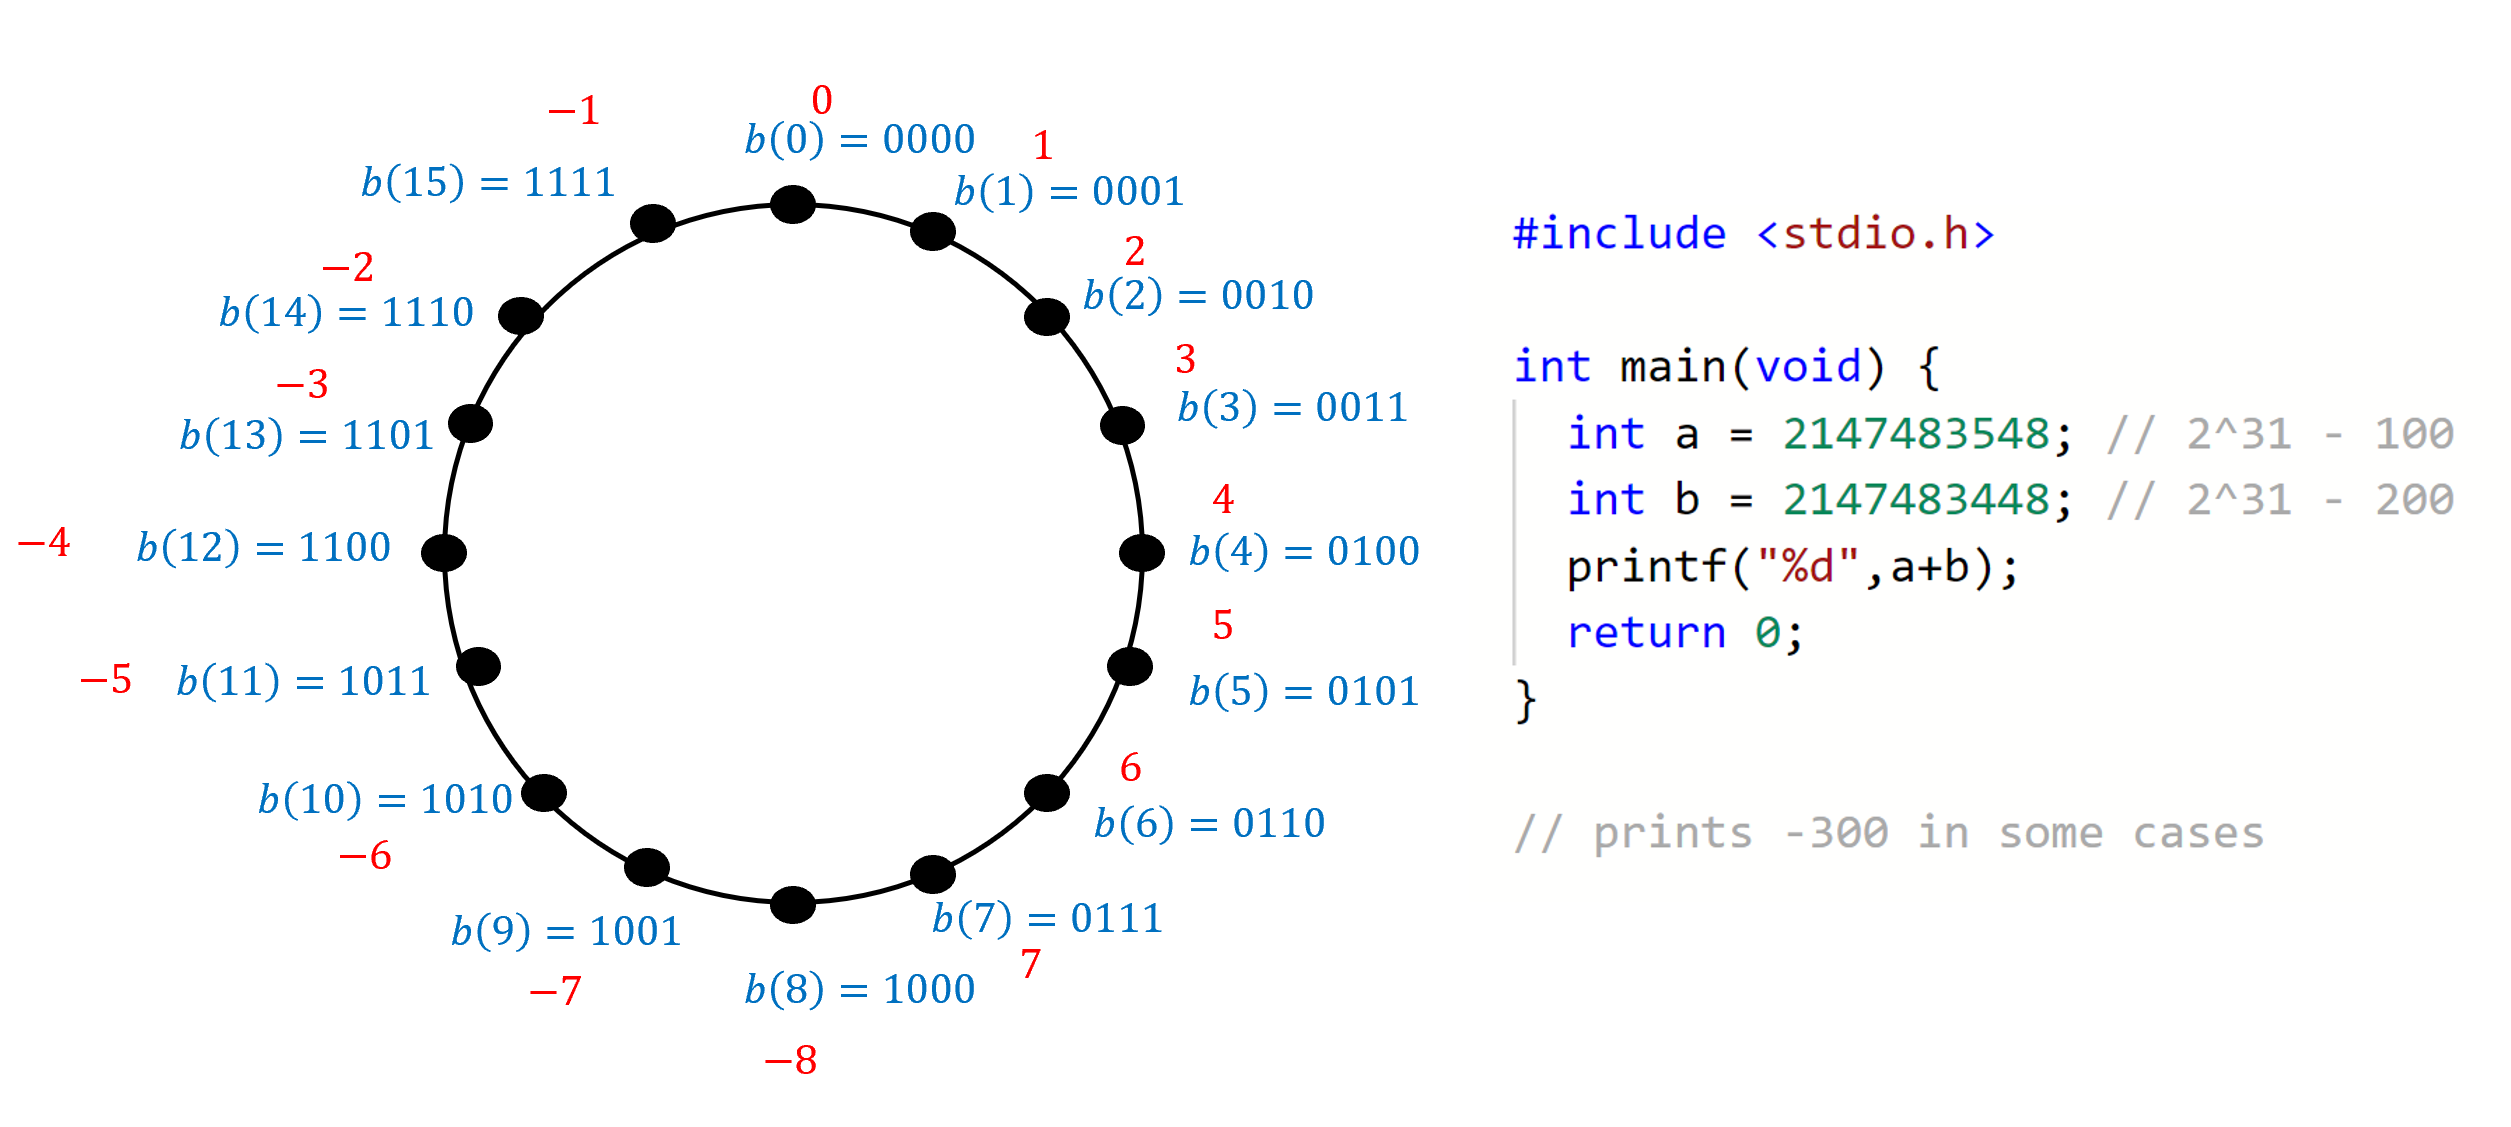
\includegraphics[width=\linewidth, height=1.5in, keepaspectratio]{../figure/twoscomplement.png}
\caption{In the \emph{two's complement representation} we represent a
potentially negative integer \(k \in \{ -2^n ,\ldots, 2^n-1 \}\) as an
\(n+1\) length string using the binary representation of the integer
\(k \mod 2^{n+1}\). On the lefthand side: this representation for
\(n=3\) (the red integers are the numbers being represented by the blue
binary strings). If a microprocessor does not check for overflows,
adding the two positive numbers \(6\) and \(5\) might result in the
negative number \(-5\) (since \(-5 \mod 16 = 11\). The righthand side is
a \texttt{C} program that will on some \(32\) bit architecture print a
negative number after adding two positive numbers. (Integer overflow in
\texttt{C} is considered \emph{undefined behavior} which means the
result of this program, including whether it runs or crashes, could
differ depending on the architecture, compiler, and even compiler
options and version.)}
\label{twoscomplementfig}
\end{marginfigure}

\subsection{Rational numbers, and representing pairs of
strings}\label{Rational-numbers-and-repr}

We can represent a rational number of the form \(a/b\) by representing
the two numbers \(a\) and \(b\). However, merely concatenating the
representations of \(a\) and \(b\) will not work. For example, the
binary representation of \(4\) is \(100\) and the binary representation
of \(43\) is \(101011\), but the concatenation \(100101011\) of these
strings is also the concatenation of the representation \(10010\) of
\(18\) and the representation \(1011\) of \(11\). Hence, if we used such
simple concatenation then we would not be able to tell if the string
\(100101011\) is supposed to represent \(4/43\) or \(18/11\).

We tackle this by giving a general representation for \emph{pairs of
strings}. If we were using a pen and paper, we would just use a
separator symbol such as \(\|\) to represent, for example, the pair
consisting of the numbers represented by \(10\) and \(110001\) as the
length-\(9\) string ``\(01\|110001\)''. In other words, there is a one
to one map \(F\) from \emph{pairs of strings} \(x,y \in \{0,1\}^*\) into
a single string \(z\) over the alphabet \(\Sigma = \{0,1,\| \}\) (in
other words, \(z\in \Sigma^*\)). Using such separators is similar to the
way we use spaces and punctuation to separate words in English. By
adding a little redundancy, we achieve the same effect in the digital
domain. We can map the three-element set \(\Sigma\) to the three-element
set \(\{00,11,01 \} \subset \{0,1\}^2\) in a one-to-one fashion, and
hence encode a length \(n\) string \(z\in \Sigma^*\) as a length \(2n\)
string \(w\in \{0,1\}^*\).

Our final representation for rational numbers is obtained by composing
the following steps:

\begin{enumerate}
\def\labelenumi{\arabic{enumi}.}
\item
  Representing a non-negative rational number as a pair of natural
  numbers.
\item
  Representing a natural number by a string via the binary
  representation.
\item
  Combining 1 and 2 to obtain a representation of a rational number as a
  pair of strings.
\item
  Representing a pair of strings over \(\{0,1\}\) as a single string
  over \(\Sigma = \{0,1,\|\}\).
\item
  Representing a string over \(\Sigma\) as a longer string over
  \(\{0,1\}\).
\end{enumerate}

\hypertarget{represnumberbypairs}{}
\begin{example}[Representing a rational number as a string] \label[example]{represnumberbypairs}

Consider the rational number \(r=-5/8\). We represent \(-5\) as \(1101\)
and \(+8\) as \(01000\), and so we can represent \(r\) as the
\emph{pair} of strings \((1101,01000)\) and represent this pair as the
length \(10\) string \(1101\|01000\) over the alphabet \(\{0,1,\|\}\).
Now, applying the map \(0 \mapsto 00\), \(1\mapsto 11\),
\(\| \mapsto 01\), we can represent the latter string as the length
\(20\) string \(s=11110011010011000000\) over the alphabet \(\{0,1\}\).

\end{example}

The same idea can be used to represent triples of strings, quadruples,
and so on as a string. Indeed, this is one instance of a very general
principle that we use time and again in both the theory and practice of
computer science (for example, in Object Oriented programming):

\hypertarget{representtuplesidea}{}
\begin{bigidea} \label[bigidea]{representtuplesidea}

If we can represent objects of type \(T\) as strings, then we can
represent tuples of objects of type \(T\) as strings as well.

\end{bigidea}

Repeating the same idea, once we can represent objects of type \(T\), we
can also represent \emph{lists of lists} of such objects, and even lists
of lists of lists and so on and so forth. We will come back to this
point when we discuss \emph{prefix free encoding} in
\cref{prefixfreesec}.

\section{Representing real numbers}\label{Representing-real-numbers}

The set of \emph{real numbers} \(\R\) contains all numbers including
positive, negative, and fractional, as well as \emph{irrational} numbers
such as \(\pi\) or \(e\). Every real number can be approximated by a
rational number, and thus we can represent every real number \(x\) by a
rational number \(a/b\) that is very close to \(x\). For example, we can
represent \(\pi\) by \(22/7\) within an error of about \(10^{-3}\). If
we want a smaller error (e.g., about \(10^{-4}\)) then we can use
\(311/99\), and so on and so forth.


\begin{figure}
\centering
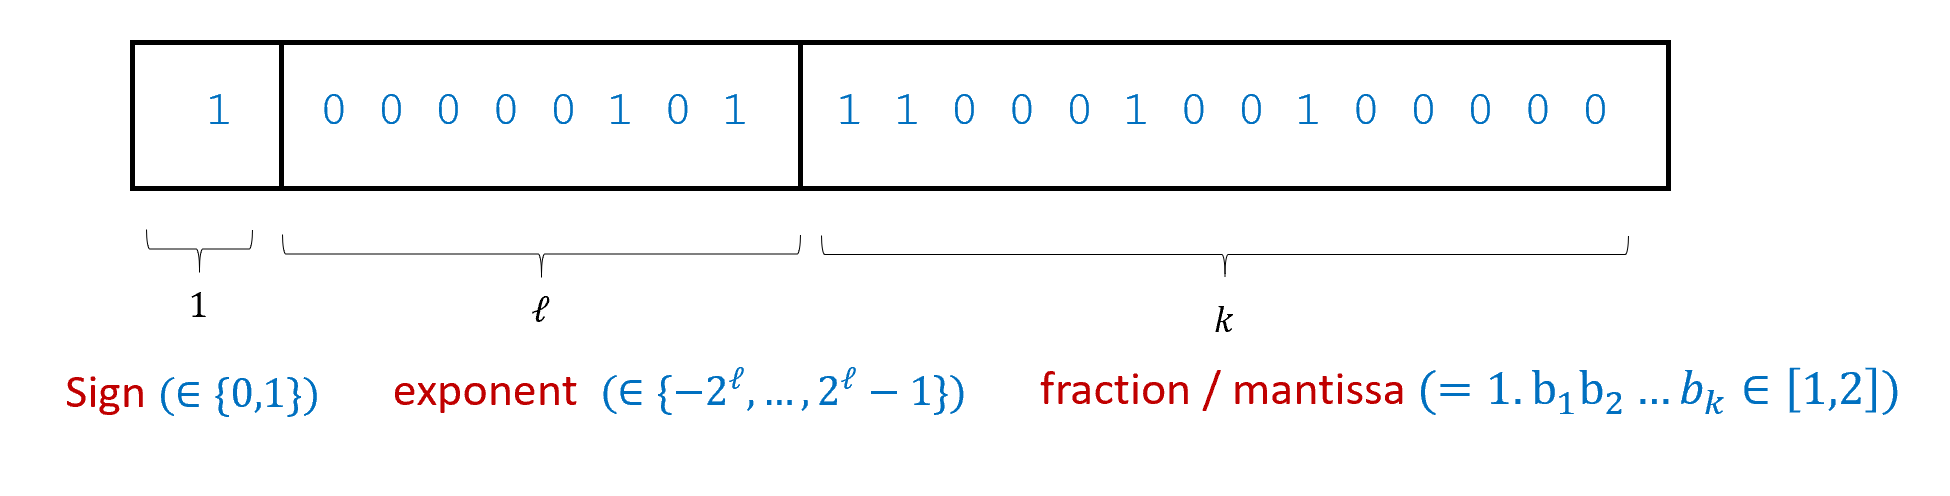
\includegraphics[width=\textwidth, height=0.25\paperheight, keepaspectratio]{../figure/floatingpoint.png}
\caption{The \emph{floating point representation} of a real number
\(x\in \R\) is its approximation as a number of the form
\(\sigma b \cdot 2^e\) where \(\sigma \in \{\pm 1 \}\), \(e\) is an
(potentially negative) integer, and \(b\) is a rational number between
\(1\) and \(2\) expressed as a binary fraction
\(1.b_0b_1b_2\ldots b_{k}\) for some \(b_1,\ldots,b_k \in \{0,1\}\)
(that is \(b = 1 + b_1/2 + b_2/4 + \ldots + b_k/2^k\)). Commonly-used
floating point representations fix the numbers \(\ell\) and \(k\) of
bits to represent \(e\) and \(b\) respectively. In the example above,
assuming we use two's complement representation for \(e\), the number
represented is
\(-1 \times 2^{5} \times ( 1 + 1/2 + 1/4 + 1/64 + 1/512) = -56.5625\).}
\label{floatingpointfig}
\end{figure}

The above representation of real numbers via rational numbers that
approximate them is a fine choice for a representation scheme. However,
typically in computing applications, it is more common to use the
\emph{floating point representation scheme} (see
\cref{floatingpointfig}) to represent real numbers. In the floating
point representation scheme we represent \(x\in \R\) by the pair
\((b,e)\) of (positive or negative) integers of some prescribed sizes
(determined by the desired accuracy) such that \(b \times 2^{e}\) is
closest to \(x\). Floating point representation is the base-two version
of \href{https://goo.gl/MUJnVE}{scientific notation}, where one
represents a number \(y\in R\) as its approximation of the form
\(b \times 10^e\) for \(b,e\). It is called ``floating point'' because
we can think of the number \(b\) as specifying a sequence of binary
digits, and \(e\) as describing the location of the ``binary point''
within this sequence. The use of floating representation is the reason
why in many programming systems, printing the expression
\texttt{0.1+0.2} will result in \texttt{0.30000000000000004} and not
\texttt{0.3}, see \href{http://floating-point-gui.de/}{here},
\href{https://docs.oracle.com/cd/E19957-01/806-3568/ncg_goldberg.html}{here}
and
\href{https://randomascii.wordpress.com/2012/04/05/floating-point-complexities/}{here}
for more.


\begin{marginfigure}
\centering
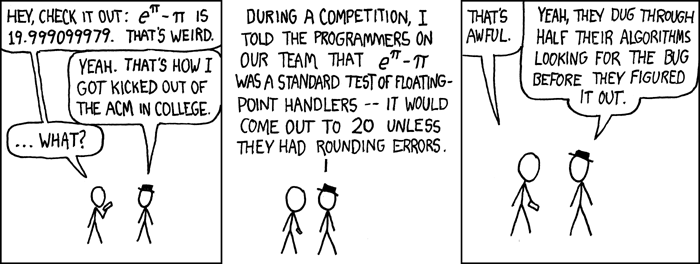
\includegraphics[width=\linewidth, height=1.5in, keepaspectratio]{../figure/e_to_the_pi_minus_pi.png}
\caption{XKCD cartoon on floating-point arithmetic.}
\label{xkcdfloatingfig}
\end{marginfigure}

The reader might be (rightly) worried about the fact that the floating
point representation (or the rational number one) can only
\emph{approximately} represent real numbers. In many (though not all)
computational applications, one can make the accuracy tight enough so
that this does not affect the final result, though sometimes we do need
to be careful. Indeed, floating-point bugs can sometimes be no joking
matter. For example, floating point rounding errors have been implicated
in the
\href{http://embeddedgurus.com/barr-code/2014/03/lethal-software-defects-patriot-missile-failure/}{failure}
of a U.S. Patriot missile to intercept an Iraqi Scud missile, costing 28
lives, as well as a 100 million pound error in computing
\href{https://catless.ncl.ac.uk/Risks/5/74}{payouts to British
pensioners}.

\subsection{Can we represent reals \emph{exactly}?}\label{cantorsec}

Given the issues with floating point approximations for real numbers, a
natural question is whether it is possible to represent real numbers
\emph{exactly} as strings. Unfortunately, the following theorem shows
that this cannot be done:

\hypertarget{cantorthm}{}
\begin{theorem}[Reals are uncountable] \label[theorem]{cantorthm}

There does not exist a one-to-one function
\(RtS:\R \rightarrow \{0,1\}^*\).\footnote{\(RtS\) stands for ``real
  numbers to strings''.}

\end{theorem}

\cref{cantorthm} was proven by
\href{https://en.wikipedia.org/wiki/Georg_Cantor}{Georg Cantor} in 1874.
(Cantor used the set \(\N\) rather than \(\{0,1\}^*\), but one can show
that these two results are equivalent using the one-to-one mappings
between those two sets, see \cref{naturalsstringsmapex}.) The
non-existence of such a map is equivalent to saying that there is no way
to ``count'' all the real numbers as some sequence
\(x_0,x_1,x_2,\ldots\). For this reason \cref{cantorthm} is known as the
\emph{uncountability of the reals}.

This result (and the theory around it) was quite shocking to
mathematicians at the time. By showing that there is no one-to-one map
from \(\R\) to \(\{0,1\}^*\) (or \(\N\)), Cantor showed that these two
infinite sets have ``different forms of infinity'' and that the set of
real numbers \(\R\) is in some sense ``bigger'' than the infinite set
\(\{0,1\}^*\). The notion that there are ``shades of infinity'' was
deeply disturbing to mathematicians and philosophers at the time. The
philosopher Ludwig Wittgenstein (whom we mentioned before) called
Cantor's results ``utter nonsense'' and ``laughable.'' Others thought
they were even worse than that. Leopold Kronecker called Cantor a
``corrupter of youth,'' while Henri Poincaré said that Cantor's ideas
``should be banished from mathematics once and for all.'' The tide
eventually turned, and these days Cantor's work is universally accepted
as the cornerstone of set theory and the foundations of mathematics. As
David Hilbert said in 1925, \emph{``No one shall expel us from the
paradise which Cantor has created for us.''} As we will see later in
this book, Cantor's ideas also play a huge role in the theory of
computation.

Now that we have discussed \cref{cantorthm}'s importance, let us see the
proof. It is achieved in two steps:

\begin{enumerate}
\def\labelenumi{\arabic{enumi}.}
\item
  Define some infinite set \(\mathcal{X}\) for which it is easier for us
  to prove that \(\mathcal{X}\) is not countable (namely, it's easier
  for us to prove that there is no one-to-one function from
  \(\mathcal{X}\) to \(\{0,1\}^*\)).
\item
  Prove that there \emph{is} a one-to-one function \(G\) mapping
  \(\mathcal{X}\) to \(\mathbb{R}\).
\end{enumerate}

We can use a proof by contradiction to show that these two facts
together imply \cref{cantorthm}. Specifically, if we assume (towards the
sake of contradiction) that there exists some one-to-one \(F\) mapping
\(\mathbb{R}\) to \(\{0,1\}^*\) then the function \(x \mapsto F(G(x))\)
obtained by composing \(F\) with the function \(G\) from Step 2 above
would be a one-to-one function from \(\mathcal{X}\) to \(\{0,1\}^*\),
which contradicts what we proved in Step 1!

To turn this idea into a full proof of \cref{cantorthm} we need to:

\begin{itemize}
\item
  Define the set \(\mathcal{X}\).
\item
  Prove that there is no one-to-one function from \(\mathcal{X}\) to
  \(\{0,1\}^*\)
\item
  Prove that there \emph{is} a one-to-one function from \(\mathcal{X}\)
  to \(\R\).
\end{itemize}

We now proceed to do precisely that. That is, we will define the set
\(\{0,1\}^\infty\), which will play the role of \(\mathcal{X}\), and
then state and prove two lemmas that show that this set satisfies our
two desired properties.

\hypertarget{bitsinfdef}{}
\begin{definition} \label[definition]{bitsinfdef}

We denote by \(\{0,1\}^\infty\) the set
\(\{ f \;|\; f:\N \rightarrow \{0,1\} \}\).

\end{definition}

That is, \(\{0,1\}^\infty\) is a set of \emph{functions}, and a function
\(f\) is in \(\{0,1\}^\infty\) iff its domain is \(\N\) and its codomain
is \(\{0,1\}\). We can also think of \(\{0,1\}^\infty\) as the set of
all infinite \emph{sequences} of bits, since a function
\(f:\N \rightarrow \{0,1\}\) can be identified with the sequence
\((f(0),f(1),f(2),\ldots )\). The following two lemmas show that
\(\{0,1\}^\infty\) can play the role of \(\mathcal{X}\) to establish
\cref{cantorthm}.

\hypertarget{sequencestostrings}{}
\begin{lemma} \label[lemma]{sequencestostrings}

There does not exist a one-to-one map
\(FtS:\{0,1\}^\infty \rightarrow \{0,1\}^*\).\footnote{\(FtS\) stands
  for ``functions to strings''.}

\end{lemma}

\hypertarget{sequencestoreals}{}
\begin{lemma} \label[lemma]{sequencestoreals}

There \emph{does} exist a one-to-one map
\(FtR:\{0,1\}^\infty \rightarrow \R\).\footnote{\(FtR\) stands for
  ``functions to reals.''}

\end{lemma}

As we've seen above, \cref{sequencestostrings} and
\cref{sequencestoreals} together imply \cref{cantorthm}. To repeat the
argument more formally, suppose, for the sake of contradiction, that
there did exist a one-to-one function \(RtS:\R \rightarrow \{0,1\}^*\).
By \cref{sequencestoreals}, there exists a one-to-one function
\(FtR:\{0,1\}^\infty \rightarrow \R\). Thus, under this assumption,
since the composition of two one-to-one functions is one-to-one (see
\cref{onetoonecompex}), the function
\(FtS:\{0,1\}^\infty \rightarrow \{0,1\}^*\) defined as
\(FtS(f)=RtS(FtR(f))\) will be one to one, contradicting
\cref{sequencestostrings}. See \cref{proofofcantorfig} for a graphical
illustration of this argument.


\begin{figure}
\centering
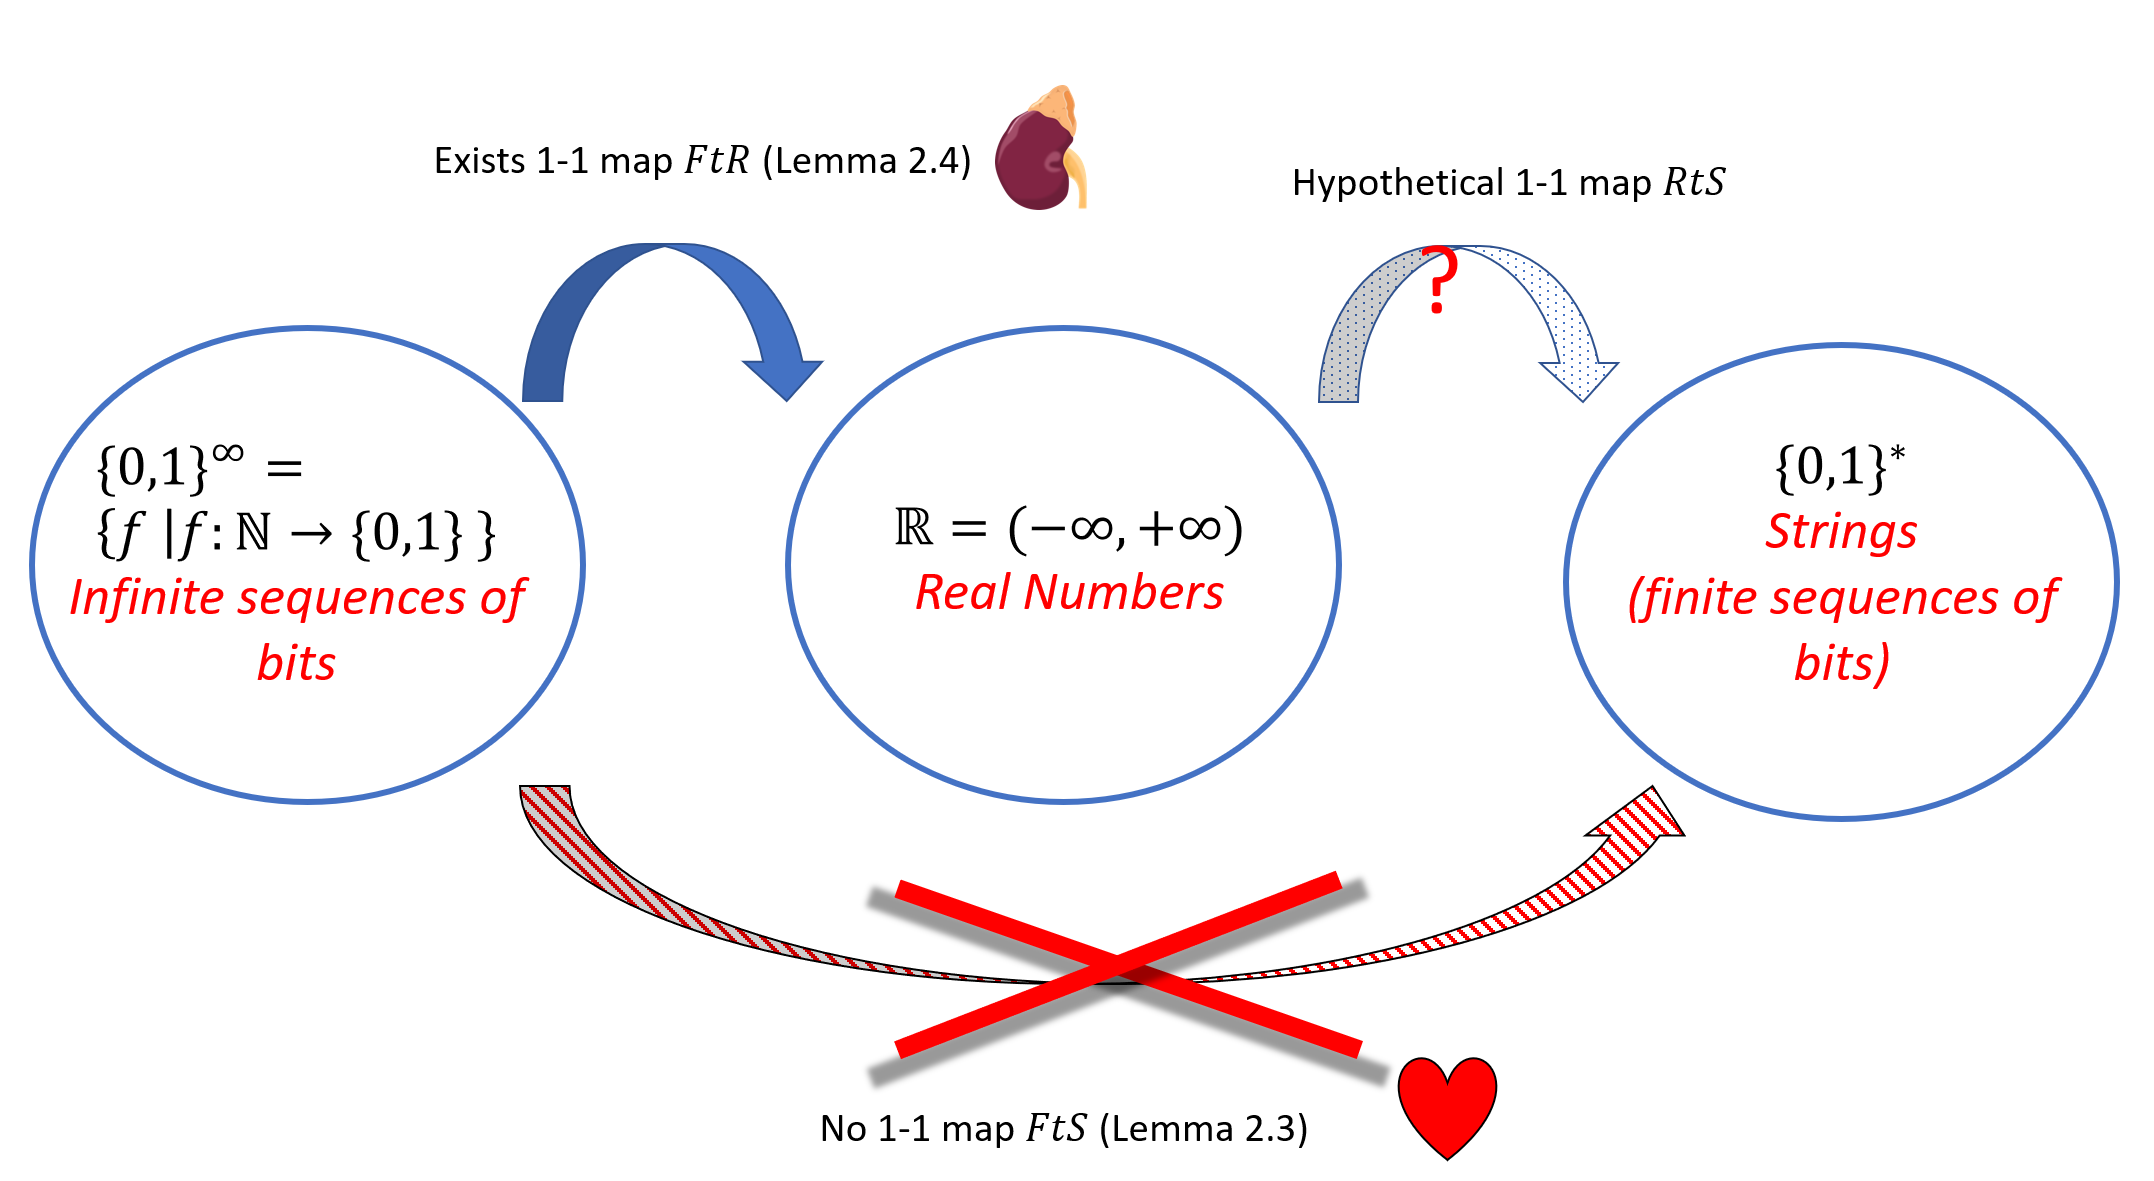
\includegraphics[width=\textwidth, height=0.25\paperheight, keepaspectratio]{../figure/proofofcantor.png}
\caption{We prove \cref{cantorthm} by combining
\cref{sequencestostrings} and \cref{sequencestoreals}.
\cref{sequencestoreals}, which uses standard calculus tools, shows the
existence of a one-to-one map \(FtR\) from the set \(\{0,1\}^\infty\) to
the real numbers. So, if a hypothetical one-to-one map
\(RtS:\R \rightarrow \{0,1\}^*\) existed, then we could compose them to
get a one-to-one map \(FtS:\{0,1\}^\infty \rightarrow \{0,1\}^*\). Yet
this contradicts \cref{sequencestostrings}- the heart of the proof-
which rules out the existence of such a map.}
\label{proofofcantorfig}
\end{figure}

Now all that is left is to prove these two lemmas. We start by proving
\cref{sequencestostrings} which is really the heart of \cref{cantorthm}.


\begin{figure}
\centering
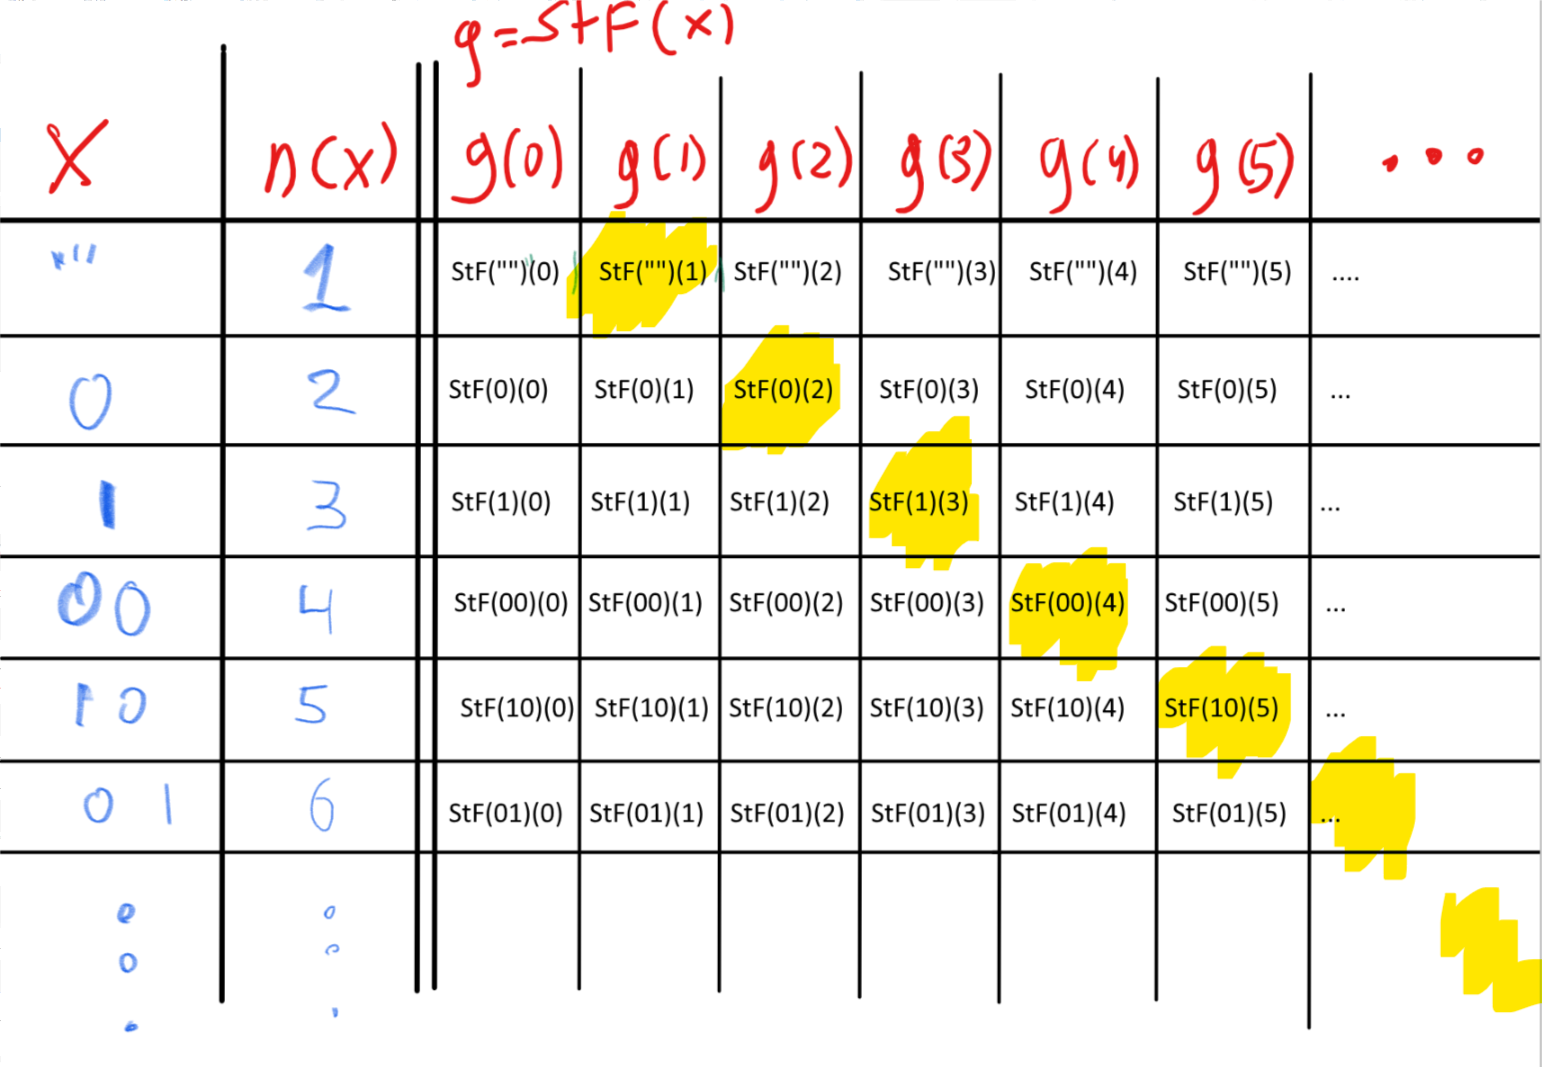
\includegraphics[width=\textwidth, height=0.25\paperheight, keepaspectratio]{../figure/diagreals2.png}
\caption{We construct a function \(\overline{d}\) such that
\(\overline{d} \neq StF(x)\) for every \(x\in \{0,1\}^*\) by ensuring
that \(\overline{d}(n(x)) \neq StF(x)(n(x))\) for every
\(x\in \{0,1\}^*\) with lexicographic order \(n(x)\). We can think of
this as building a table where the columns correspond to numbers
\(m\in \N\) and the rows correspond to \(x\in \{0,1\}^*\) (sorted
according to \(n(x)\)). If the entry in the \(x\)-th row and the
\(m\)-th column corresponds to \(g(m))\) where \(g=StF(x)\) then
\(\overline{d}\) is obtained by going over the ``diagonal'' elements in
this table (the entries corresponding to the \(x\)-th row and
\(n(x)\)-th column) and ensuring that
\(\overline{d}(x)(n(x)) \neq StF(x)(n(x))\).}
\label{diagrealsfig}
\end{figure}

\begin{proof}[Proof of \cref{sequencestostrings}] \label[proof]{We-will-prove-that-there-}

We will prove that there does not exist an \emph{onto} function
\(StF:\{0,1\}^* \rightarrow \{0,1\}^\infty\). This implies the lemma
since for every two sets \(A\) and \(B\), there exists an onto function
from \(A\) to \(B\) if and only if there exists a one-to-one function
from \(B\) to \(A\) (see \cref{onetooneimpliesonto}).

The technique of this proof is known as the ``diagonal argument'' and is
illustrated in \cref{diagrealsfig}. We assume, towards a contradiction,
that there exists such a function
\(StF:\{0,1\}^* \rightarrow \{0,1\}^\infty\). We will show that \(StF\)
is not onto by demonstrating a function
\(\overline{d}\in \{0,1\}^\infty\) such that
\(\overline{d} \neq StF(x)\) for every \(x\in \{0,1\}^*\). Consider the
lexicographic ordering of binary strings (i.e.,
\(\ensuremath{\text{\texttt{""}}}\),\(0\),\(1\),\(00\),\(01\),\(\ldots\)).
For every \(n\in \N\), we let \(x_n\) be the \(n\)-th string in this
order. That is \(x_0 =\ensuremath{\text{\texttt{""}}}\), \(x_1 = 0\),
\(x_2= 1\) and so on and so forth. We define the function
\(\overline{d} \in \{0,1\}^\infty\) as follows:
\[\overline{d}(n) = 1 - StF(x_n)(n)\] for every \(n\in \N\). That is, to
compute \(\overline{d}\) on input \(n\in\N\), we first compute
\(g= StF(x_n)\), where \(x_n \in \{0,1\}^*\) is the \(n\)-th string in
the lexicographical ordering. Since \(g \in \{0,1\}^\infty\), it is a
function mapping \(\N\) to \(\{0,1\}\). The value \(\overline{d}(n)\) is
defined to be the negation of \(g(n)\).

The definition of the function \(\overline{d}\) is a bit subtle. One way
to think about it is to imagine the function \(StF\) as being specified
by an infinitely long table, in which every row corresponds to a string
\(x\in \{0,1\}^*\) (with strings sorted in lexicographic order), and
contains the sequence \(StF(x)(0), StF(x)(1), StF(x)(2),\ldots\). The
\emph{diagonal} elements in this table are the values

\[StF(\ensuremath{\text{\texttt{""}}})(0),StF(0)(1),StF(1)(2),StF(00)(3), StF(01)(4),\ldots\]

which correspond to the elements \(StF(x_n)(n)\) in the \(n\)-th row and
\(n\)-th column of this table for \(n=0,1,2,\ldots\). The function
\(\overline{d}\) we defined above maps every \(n\in \N\) to the negation
of the \(n\)-th diagonal value.

To complete the proof that \(StF\) is not onto we need to show that
\(\overline{d} \neq StF(x)\) for every \(x\in \{0,1\}^*\). Indeed, let
\(x\in \{0,1\}^*\) be some string and let \(g = StF(x)\). If \(n\) is
the position of \(x\) in the lexicographical order then by construction
\(\overline{d}(n) = 1-g(n) \neq g(n)\) which means that
\(g \neq \overline{d}\) which is what we wanted to prove.

\end{proof}

\begin{pause} \label[pause]{The-proof-of-crefsequence}

The proof of \cref{sequencestostrings} is rather subtle, and worth
re-reading a second or third time. We will use the ``diagonal argument''
again several times later on in this book.

\end{pause}

\hypertarget{generalizepowerset}{}
\begin{remark}[Generalizing beyond strings and reals] \label[remark]{generalizepowerset}

\cref{sequencestostrings} doesn't really have much to do with the
natural numbers or the strings. An examination of the proof shows that
it really shows that for \emph{every} set \(S\), there is no one-to-one
map \(F:\{0,1\}^S \rightarrow S\) where \(\{0,1\}^S\) denotes the set
\(\{ f \;|\; f:S \rightarrow \{0,1\} \}\) of all Boolean functions with
domain \(S\). Since we can identify a subset \(V \subseteq S\) with its
characteristic function \(f=1_V\) (i.e., \(1_V(x)=1\) iff \(x\in V\)),
we can think of \(\{0,1\}^S\) also as the set of all \emph{subsets} of
\(S\). This subset is sometimes called the \emph{power set} of \(S\).

The proof of \cref{sequencestostrings} can be generalized to show that
there is no one-to-one map between a set and its power set. In
particular, it means that the set \(\{0,1\}^\R\) is ``even bigger'' than
\(\R\). Cantor used these ideas to construct an infinite hierarchy of
shades of infinity. The number of such shades turns out to be much
larger than \(|\N|\) or even \(|\R|\). He denoted the cardinality of
\(\N\) by \(\aleph_0\) and denoted the next largest infinite number by
\(\aleph_1\). (\(\aleph\) is the first letter in the Hebrew alphabet.)
Cantor also made the
\href{https://en.wikipedia.org/wiki/Continuum_hypothesis}{continuum
hypothesis} that \(|\R|=\aleph_1\). We will come back to the fascinating
story of this hypothesis later on in this book.
\href{https://www.scottaaronson.com/democritus/lec2.html}{This lecture
of Aaronson} mentions some of these issues (see also
\href{http://www.eecs70.org/static/notes/n10.pdf}{this Berkeley CS 70
lecture}).

\end{remark}

To complete the proof of \cref{cantorthm}, we need to show
\cref{sequencestoreals}. This requires some calculus background but is
otherwise straightforward. If you have not had much experience with
limits of a real series before, then the formal proof below might be a
little hard to follow. This part is not the core of Cantor's argument,
nor are such limits important to the remainder of this book, so you can
feel free to take \cref{sequencestoreals} on faith and skip the proof.

\begin{proofidea} \label[proofidea]{We-define-FtRf-to-be-the-}

We define \(FtR(f)\) to be the number between \(0\) and \(2\) whose
decimal expansion is \(f(0).f(1) f(2) \ldots\), or in other words
\(FtR(f) = \sum_{i=0}^{\infty} f(i) \cdot 10^{-i}\). To prove that
\(FtR\) is one to one, we need to show that if \(f \neq g\) then
\(FtR(f) \neq FtR(g)\). To do that we let \(k\in \N\) be the first input
on which \(f\) and \(g\) disagree. The numbers \(FtR(f)\) and \(FtR(g)\)
agree in the first \(k-1\) digits following the decimal point and
disagree in the \(k\)-th digit. One can then calculate and verify that
this means that \(|FtR(f)-FtR(g)| > 0.5 \cdot 10^{-k}\) which in
particular means that these two numbers are distinct from one another.
(You might wonder why we can't immediately deduce that two numbers that
differ in a digit are not the same. The issue is that we have to be a
little more careful when talking about infinite expansions. For example,
the number one half has two decimal expansions \(0.5\) and
\(0.49999\cdots\). However, this issue does not come up if (as in our
case) we restrict attention only to numbers with decimal expansions that
do not involve the digit \(9\).)

\end{proofidea}

\begin{proof}[Proof of \cref{sequencestoreals}] \label[proof]{For-every-f-in-infty-we-d}

For every \(f \in \{0,1\}^\infty\), we define \(FtR(f)\) to be the
number whose decimal expansion is \(f(0).f(1)f(2)f(3)\ldots\).

Formally we define \[
FtR(f) = \sum_{i=0}^\infty f(i) \cdot 10^{-i} \label{eqcantordecimalexpansion}
\] It is a known result in calculus (whose proof we will not repeat
here) that the series on the righthand side of
\eqref{eqcantordecimalexpansion} converges to a definite limit in
\(\mathbb{R}\).

We now prove that \(FtR\) is one to one. Let \(f,g\) be two distinct
functions in \(\{0,1\}^\infty\). Since \(f\) and \(g\) are distinct,
there must be some input on which they differ, and we define \(k\) to be
the smallest such input and assume without loss of generality that
\(f(k)=0\) and \(g(k)=1\). (Otherwise, if \(f(k)=1\) and \(g(k)=0\),
then we can simply switch the roles of \(f\) and \(g\).) The numbers
\(FtR(f)\) and \(FtR(g)\) agree with each other up to the \(k-1\)-th
digit up after the decimal point. Since this digit equals \(0\) for
\(FtR(f)\) and equals \(1\) for \(FtR(g)\), we claim that \(FtR(g)\) is
bigger than \(FtR(f)\) by at least \(0.5 \cdot 10^{-k}\). To see this
note that the difference \(FtR(g)-FtR(f)\) will be minimized if
\(g(\ell)=0\) for every \(\ell>k\) and \(f(\ell)=1\) for every
\(\ell>k\), in which case (since \(f\) and \(g\) agree up to the
\(k-1\)-th digit)

\[
FtR(g)-FtR(f) = 10^{-k} - 10^{-k-1} - 10^{-k-2} - 10^{-k-3} - \cdots \label{eqcantordecimalexpansion}
\]

Since the infinite series \(\sum_{j=0}^{\infty} 10^{-i}\) converges to
\(10/9\), it follows that for every such \(f\) and \(g\),
\(FtR(g) - FtR(f) \geq 10^{-k} - 10^{-k-1}\cdot (10/9) > 0\). In
particular we see that for every distinct \(f,g \in \{0,1\}^\infty\),
\(FtR(f) \neq FtR(g)\), implying that the function \(FtR\) is one to
one.

\end{proof}

\hypertarget{decimal}{}
\begin{remark}[Using decimal expansion (optional)] \label[remark]{decimal}

In the proof above we used the fact that \(1 + 1/10 + 1/100 + \cdots\)
converges to \(10/9\), which plugging into
\eqref{eqcantordecimalexpansion} yields that the difference between
\(FtR(g)\) and \(FtR(h)\) is at least
\(10^{-k} - 10^{-k-1}\cdot (10/9) > 0\). While the choice of the decimal
representation for \(FtR\) was arbitrary, we could not have used the
binary representation in its place. Had we used the \emph{binary}
expansion instead of decimal, the corresponding sequence
\(1 + 1/2 + 1/4 + \cdots\) converges to \(2/1=2\), and since
\(2^{-k} = 2^{-k-1} \cdot 2\), we could not have deduced that \(FtR\) is
one to one. Indeed there do exist pairs of distinct sequences
\(f,g\in \{0,1\}^\infty\) such that
\(\sum_{i=0}^\infty f(i)2^{-i} = \sum_{i=0}^\infty g(i)2^{-i}\). (For
example, the sequence \(1,0,0,0,\ldots\) and the sequence
\(0,1,1,1,\ldots\) have this property.)

\end{remark}

\section{Representing objects beyond
numbers}\label{Representing-objects-beyo}

Numbers are of course by no means the only objects that we can represent
as binary strings. A \emph{representation scheme} for representing
objects from some set \(\mathcal{O}\) consists of an \emph{encoding}
function that maps an object in \(\mathcal{O}\) to a string, and a
\emph{decoding} function that decodes a string back to an object in
\(\mathcal{O}\). Formally, we make the following definition:

\hypertarget{binaryrepdef}{}
\begin{definition}[String representation] \label[definition]{binaryrepdef}

Let \(\mathcal{O}\) be any set. A \emph{representation scheme} for
\(\mathcal{O}\) is a pair of functions \(E,D\) where
\(E:\mathcal{O} \rightarrow \{0,1\}^*\) is a total one-to-one function,
\(D:\{0,1\}^* \rightarrow_p \mathcal{O}\) is a (possibly partial)
function, and such that \(D\) and \(E\) satisfy that \(D(E(o))=o\) for
every \(o\in \mathcal{O}\). \(E\) is known as the \emph{encoding}
function and \(D\) is known as the \emph{decoding} function.

\end{definition}

Note that the condition \(D(E(o))=o\) for every \(o\in\mathcal{O}\)
implies that \(D\) is \emph{onto} (can you see why?). It turns out that
to construct a representation scheme we only need to find an
\emph{encoding} function. That is, every one-to-one encoding function
has a corresponding decoding function, as shown in the following lemma:

\hypertarget{decodelem}{}
\begin{lemma} \label[lemma]{decodelem}

Suppose that \(E: \mathcal{O} \rightarrow \{0,1\}^*\) is one-to-one.
Then there exists a function \(D:\{0,1\}^* \rightarrow \mathcal{O}\)
such that \(D(E(o))=o\) for every \(o\in \mathcal{O}\).

\end{lemma}

\begin{proof} \label[proof]{Let-o-be-some-arbitrary-e}

Let \(o_0\) be some arbitrary element of \(\mathcal{O}\). For every
\(x \in \{0,1\}^*\), there exists either zero or a single
\(o\in \mathcal{O}\) such that \(E(o)=x\) (otherwise \(E\) would not be
one-to-one). We will define \(D(x)\) to equal \(o_0\) in the first case
and this single object \(o\) in the second case. By definition
\(D(E(o))=o\) for every \(o\in \mathcal{O}\).

\end{proof}

\hypertarget{totaldecoding}{}
\begin{remark}[Total decoding functions] \label[remark]{totaldecoding}

While the decoding function of a representation scheme can in general be
a \emph{partial} function, the proof of \cref{decodelem} implies that
every representation scheme has a \emph{total} decoding function. This
observation can sometimes be useful.

\end{remark}

\subsection{Finite representations}\label{Finite-representations}

If \(\mathcal{O}\) is \emph{finite}, then we can represent every object
in \(\mathcal{O}\) as a string of length at most some number \(n\). What
is the value of \(n\)? Let us denote by \(\{0,1\}^{\leq n}\) the set
\(\{ x\in \{0,1\}^* : |x| \leq n \}\) of strings of length at most
\(n\). The size of \(\{0,1\}^{\leq n}\) is equal to \[
|\{0,1\}^0| + |\{0,1\}^1| + |\{0,1\}^2| + \cdots + |\{0,1\}^n| = \sum_{i=0}^n 2^i = 2^{n+1}-1
\] using the standard formula for summing a
\href{https://en.wikipedia.org/wiki/Geometric_progression}{geometric
progression}.

To obtain a representation of objects in \(\mathcal{O}\) as strings of
length at most \(n\) we need to come up with a one-to-one function from
\(\mathcal{O}\) to \(\{0,1\}^{\leq n}\). We can do so, if and only if
\(|\mathcal{O}| \leq 2^{n+1}-1\) as is implied by the following lemma:

\hypertarget{onetoone}{}
\begin{lemma} \label[lemma]{onetoone}

For every two finite sets \(S,T\), there exists a one-to-one
\(E:S \rightarrow T\) if and only if \(|S| \leq |T|\).

\end{lemma}

\begin{proof} \label[proof]{Let-kS-and-mT-and-so-writ}

Let \(k=|S|\) and \(m=|T|\) and so write the elements of \(S\) and \(T\)
as \(S = \{ s_0 , s_1, \ldots, s_{k-1} \}\) and
\(T= \{ t_0 , t_1, \ldots, t_{m-1} \}\). We need to show that there is a
one-to-one function \(E: S \rightarrow T\) iff \(k \leq m\). For the
``if'' direction, if \(k \leq m\) we can simply define \(E(s_i)=t_i\)
for every \(i\in [k]\). Clearly for \(i \neq j\),
\(t_i = E(s_i) \neq E(s_j) = t_j\), and hence this function is
one-to-one. In the other direction, suppose that \(k>m\) and
\(E: S \rightarrow T\) is some function. Then \(E\) cannot be
one-to-one. Indeed, for \(i=0,1,\ldots,m-1\) let us ``mark'' the element
\(t_j=E(s_i)\) in \(T\). If \(t_j\) was marked before, then we have
found two objects in \(S\) mapping to the same element \(t_j\).
Otherwise, since \(T\) has \(m\) elements, when we get to \(i=m-1\) we
mark all the objects in \(T\). Hence, in this case, \(E(s_m)\) must map
to an element that was already marked before. (This observation is
sometimes known as the ``Pigeon Hole Principle'': the principle that if
you have a pigeon coop with \(m\) holes, and \(k>m\) pigeons, then there
must be two pigeons in the same hole. )

\end{proof}

\subsection{Prefix-free encoding}\label{prefixfreesec}

When showing a representation scheme for rational numbers, we used the
``hack'' of encoding the alphabet \(\{ 0,1, \|\}\) to represent tuples
of strings as a single string. This is a special case of the general
paradigm of \emph{prefix-free} encoding. The idea is the following: if
our representation has the property that no string \(x\) representing an
object \(o\) is a \emph{prefix} (i.e., an initial substring) of a string
\(y\) representing a different object \(o'\), then we can represent a
\emph{list} of objects by merely concatenating the representations of
all the list members. For example, because in English every sentence
ends with a punctuation mark such as a period, exclamation, or question
mark, no sentence can be a prefix of another and so we can represent a
list of sentences by merely concatenating the sentences one after the
other. (English has some complications such as periods used for
abbreviations (e.g., ``e.g.'') or sentence quotes containing
punctuation, but the high level point of a prefix-free representation
for sentences still holds.)

It turns out that we can transform \emph{every} representation to a
prefix-free form. This justifies \cref{representtuplesidea}, and allows
us to transform a representation scheme for objects of a type \(T\) to a
representation scheme of \emph{lists} of objects of the type \(T\). By
repeating the same technique, we can also represent lists of lists of
objects of type \(T\), and so on and so forth. But first let us formally
define prefix-freeness:

\hypertarget{prefixfreedef}{}
\begin{definition}[Prefix free encoding] \label[definition]{prefixfreedef}

For two strings \(y,y'\), we say that \(y\) is a \emph{prefix} of \(y'\)
if \(|y| \leq |y'|\) and for every \(i<|y|\), \(y'_i = y_i\).

Let \(\mathcal{O}\) be a non-empty set and
\(E:\mathcal{O} \rightarrow \{0,1\}^*\) be a function. We say that \(E\)
is \emph{prefix-free} if \(E(o)\) is non-empty for every
\(o\in\mathcal{O}\) and there does not exist a distinct pair of objects
\(o, o' \in \mathcal{O}\) such that \(E(o)\) is a prefix of \(E(o')\).

\end{definition}

Recall that for every set \(\mathcal{O}\), the set \(\mathcal{O}^*\)
consists of all finite length tuples (i.e., \emph{lists}) of elements in
\(\mathcal{O}\). The following theorem shows that if \(E\) is a
prefix-free encoding of \(\mathcal{O}\) then by concatenating encodings
we can obtain a valid (i.e., one-to-one) representation of
\(\mathcal{O}^*\):

\hypertarget{prefixfreethm}{}
\begin{theorem}[Prefix-free implies tuple encoding] \label[theorem]{prefixfreethm}

Suppose that \(E:\mathcal{O} \rightarrow \{0,1\}^*\) is prefix-free.
Then the following map
\(\overline{E}:\mathcal{O}^* \rightarrow \{0,1\}^*\) is one to one, for
every \(o_0,\ldots,o_{k-1} \in \mathcal{O}^*\), we define \[
\overline{E}(o_0,\ldots,o_{k-1}) = E(o_0)E(o_1) \cdots E(o_{k-1}) \;.
\]

\end{theorem}

\begin{pause} \label[pause]{crefprefixfreethm-is-an-e}

\cref{prefixfreethm} is an example of a theorem that is a little hard to
parse, but in fact is fairly straightforward to prove once you
understand what it means. Therefore, I highly recommend that you pause
here to make sure you understand the statement of this theorem. You
should also try to prove it on your own before proceeding further.

\end{pause}


\begin{marginfigure}
\centering
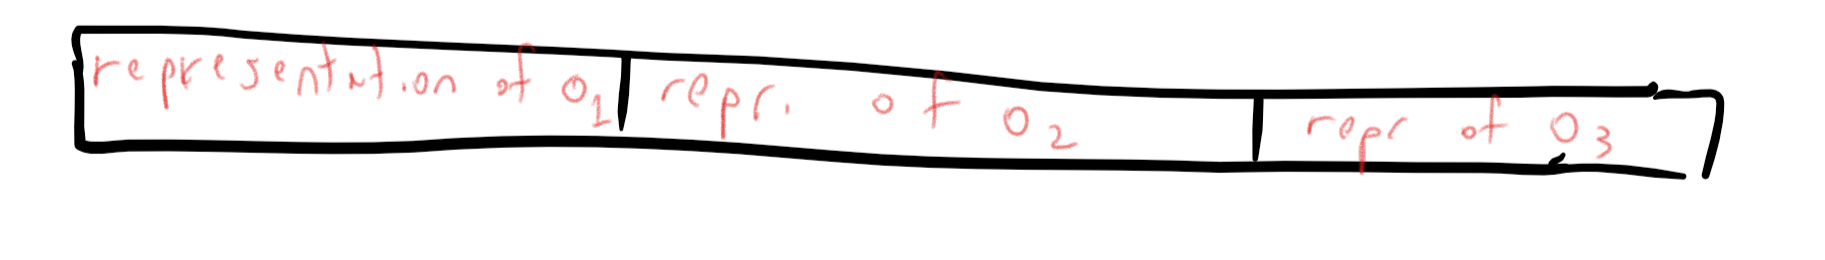
\includegraphics[width=\linewidth, height=1.5in, keepaspectratio]{../figure/repres_list.png}
\caption{If we have a prefix-free representation of each object then we
can concatenate the representations of \(k\) objects to obtain a
representation for the tuple \((o_0,\ldots,o_{k-1})\).}
\label{prefixfreerepconcat}
\end{marginfigure}

\begin{proofidea} \label[proofidea]{The-idea-behind-the-proof}

The idea behind the proof is simple. Suppose that for example we want to
decode a triple \((o_0,o_1,o_2)\) from its representation
\(x= \overline{E}(o_0,o_1,o_2)=E(o_0)E(o_1)E(o_2)\). We will do so by
first finding the first prefix \(x_0\) of \(x\) such is a representation
of some object. Then we will decode this object, remove \(x_0\) from
\(x\) to obtain a new string \(x'\), and continue onwards to find the
first prefix \(x_1\) of \(x'\) and so on and so forth (see
\cref{prefix-free-tuples-ex}). The prefix-freeness property of \(E\)
will ensure that \(x_0\) will in fact be \(E(o_0)\), \(x_1\) will be
\(E(o_1)\), etc.

\end{proofidea}

\begin{proof}[Proof of \cref{prefixfreethm}] \label[proof]{We-now-show-the-formal-pr}

We now show the formal proof. Suppose, towards the sake of
contradiction, that there exist two distinct tuples
\((o_0,\ldots,o_{k-1})\) and \((o'_0,\ldots,o'_{k'-1})\) such that

\[
\overline{E}(o_0,\ldots,o_{k-1})= \overline{E}(o'_0,\ldots,o'_{k'-1}) \;. \label{prefixfreeassump}
\] We will denote the string \(\overline{E}(o_0,\ldots,o_{k-1})\) by
\(\overline{x}\).

Let \(i\) be the first index such that \(o_i \neq o'_i\). (If
\(o_i=o'_i\) for all \(i\) then, since we assume the two tuples are
distinct, one of them must be larger than the other. In this case we
assume without loss of generality that \(k'>k\) and let \(i=k\).) In the
case that \(i<k\), we see that the string \(\overline{x}\) can be
written in two different ways:

\[
\overline{x} = \overline{E}(o_0,\ldots,o_{k-1}) = x_0\cdots x_{i-1} E(o_i) E(o_{i+1}) \cdots E(o_{k-1})
\]

and

\[
\overline{x} = \overline{E}(o'_0,\ldots,o'_{k'-1}) = x_0\cdots x_{i-1} E(o'_i) E(o'_{i+1}) \cdots E(o'_{k-1})
\]

where \(x_j = E(o_j) = E(o'_j)\) for all \(j<i\). Let \(\overline{y}\)
be the string obtained after removing the prefix \(x_0 \cdots x_{i-i}\)
from \(\overline{x}\). We see that \(\overline{y}\) can be written as
both \(\overline{y}= E(o_i)s\) for some string \(s\in \{0,1\}^*\) and as
\(\overline{y} = E(o'_i)s'\) for some \(s'\in \{0,1\}^*\). But this
means that one of \(E(o_i)\) and \(E(o'_i)\) must be a prefix of the
other, contradicting the prefix-freeness of \(E\).

In the case that \(i=k\) and \(k'>k\), we get a contradiction in the
following way. In this case

\[\overline{x} = E(o_0)\cdots E(o_{k-1}) = E(o_0) \cdots E(o_{k-1}) E(o'_k) \cdots E(o'_{k'-1})\]

which means that \(E(o'_k) \cdots E(o'_{k'-1})\) must correspond to the
empty string \(\text{\ensuremath{\text{\texttt{""}}}}\). But in such a
case \(E(o'_k)\) must be the empty string, which in particular is the
prefix of any other string, contradicting the prefix-freeness of \(E\).

\end{proof}

\hypertarget{prefixfreelistsrem}{}
\begin{remark}[Prefix freeness of list representation] \label[remark]{prefixfreelistsrem}

Even if the representation \(E\) of objects in \(\mathcal{O}\) is prefix
free, this does not mean that our representation \(\overline{E}\) of
\emph{lists} of such objects will be prefix free as well. In fact, it
won't be: for every three objects \(o,o',o''\) the representation of the
list \((o,o')\) will be a prefix of the representation of the list
\((o,o',o'')\). However, as we see in \cref{prefixfreetransformationlem}
below, we can transform \emph{every} representation into prefix-free
form, and so will be able to use that transformation if needed to
represent lists of lists, lists of lists of lists, and so on and so
forth.

\end{remark}

\subsection{Making representations
prefix-free}\label{Making-representations-pr}

Some natural representations are prefix-free. For example, every
\emph{fixed output length} representation (i.e., one-to-one function
\(E:\mathcal{O} \rightarrow \{0,1\}^n\)) is automatically prefix-free,
since a string \(x\) can only be a prefix of an equal-length \(x'\) if
\(x\) and \(x'\) are identical. Moreover, the approach we used for
representing rational numbers can be used to show the following:

\hypertarget{prefixfreetransformationlem}{}
\begin{lemma} \label[lemma]{prefixfreetransformationlem}

Let \(E:\mathcal{O} \rightarrow \{0,1\}^*\) be a one-to-one function.
Then there is a one-to-one prefix-free encoding \(\overline{E}\) such
that \(|\overline{E}(o)| \leq 2|E(o)|+2\) for every
\(o\in \mathcal{O}\).

\end{lemma}

\begin{pause} \label[pause]{For-the-sake-of-completen}

For the sake of completeness, we will include the proof below, but it is
a good idea for you to pause here and try to prove it on your own, using
the same technique we used for representing rational numbers.

\end{pause}

\begin{proof}[Proof of \cref{prefixfreetransformationlem}] \label[proof]{The-idea-behind-the-proof}

The idea behind the proof is to use the map \(0 \mapsto 00\),
\(1 \mapsto 11\) to ``double'' every bit in the string \(x\) and then
mark the end of the string by concatenating to it the pair \(01\). If we
encode a string \(x\) in this way, it ensures that the encoding of \(x\)
is never a prefix of the encoding of a distinct string \(x'\). Formally,
we define the function
\(\ensuremath{\mathit{PF}}:\{0,1\}^* \rightarrow \{0,1\}^*\) as follows:
\[\ensuremath{\mathit{PF}}(x)=x_0 x_0 x_1 x_1 \ldots x_{n-1}x_{n-1}01\]
for every \(x\in \{0,1\}^*\). If \(E:\mathcal{O} \rightarrow \{0,1\}^*\)
is the (potentially not prefix-free) representation for \(\mathcal{O}\),
then we transform it into a prefix-free representation
\(\overline{E}:\mathcal{O} \rightarrow \{0,1\}^*\) by defining
\(\overline{E}(o)=\ensuremath{\mathit{PF}}(E(o))\).

To prove the lemma we need to show that \textbf{(1)} \(\overline{E}\) is
one-to-one and \textbf{(2)} \(\overline{E}\) is prefix-free. In fact,
prefix freeness is a stronger condition than one-to-one (if two strings
are equal then in particular one of them is a prefix of the other) and
hence it suffices to prove \textbf{(2)}, which we now do.

Let \(o \neq o'\) in \(\mathcal{O}\) be two distinct objects. We will
prove that \(\overline{E}(o)\) is a not a prefix of
\(\overline{E}(o')\). Define \(x = E(o)\) and \(x'=E(o')\). Since \(E\)
is one-to-one, \(x \neq x'\). Under our assumption,
\(\ensuremath{\mathit{PF}}(x)\) is a prefix of
\(\ensuremath{\mathit{PF}}(x')\). If \(|x|<|x'|\) then the two bits in
positions \(2|x|,2|x|+1\) in \(\ensuremath{\mathit{PF}}(x)\) have the
value \(01\) but the corresponding bits in
\(\ensuremath{\mathit{PF}}(x')\) will equal either \(00\) or \(11\)
(depending on the \(|x|\)-th bit of \(x'\)) and hence
\(\ensuremath{\mathit{PF}}(x)\) cannot be a prefix of
\(\ensuremath{\mathit{PF}}(x')\). If \(|x|=|x'|\) then, since
\(x \neq x'\), there must be a coordinate \(i\) in which they differ,
meaning that the strings \(\ensuremath{\mathit{PF}}(x)\) and
\(\ensuremath{\mathit{PF}}(x')\) differ in the coordinates \(2i,2i+1\),
which again means that \(\ensuremath{\mathit{PF}}(x)\) cannot be a
prefix of \(\ensuremath{\mathit{PF}}(x')\). If \(|x|>|x'|\) then
\(|\ensuremath{\mathit{PF}}(x)|=2|x|+2>|\ensuremath{\mathit{PF}}(x')|=2|x'|+2\)
and hence \(\ensuremath{\mathit{PF}}(x)\) is longer than (and cannot be
a prefix of) \(\ensuremath{\mathit{PF}}(x')\). In all cases we see that
\(\ensuremath{\mathit{PF}}(x)=\overline{E}(o)\) is not a prefix of
\(\ensuremath{\mathit{PF}}(x')=\overline{E}(o')\), hence completing the
proof.

\end{proof}

The proof of \cref{prefixfreetransformationlem} is not the only or even
the best way to transform an arbitrary representation into prefix-free
form. \cref{prefix-free-ex} asks you to construct a more efficient
prefix-free transformation satisfying
\(|\overline{E}(o)| \leq |E(o)| + O(\log |E(o)|)\).

\subsection{``Proof by Python''
(optional)}\label{Proof-by-Python-optional}

The proofs of \cref{prefixfreethm} and
\cref{prefixfreetransformationlem} are \emph{constructive} in the sense
that they give us:

\begin{itemize}
\item
  A way to transform the encoding and decoding functions of any
  representation of an object \(O\) to encoding and decoding functions
  that are prefix-free, and
\item
  A way to extend prefix-free encoding and decoding of single objects to
  encoding and decoding of \emph{lists} of objects by concatenation.
\end{itemize}

Specifically, we could transform any pair of Python functions
\texttt{encode} and \texttt{decode} to functions \texttt{pfencode} and
\texttt{pfdecode} that correspond to a prefix-free encoding and
decoding. Similarly, given \texttt{pfencode} and \texttt{pfdecode} for
single objects, we can extend them to encoding of lists. Let us show how
this works for the case of the \texttt{NtS} and \texttt{StN} functions
we defined above.

We start with the ``Python proof'' of
\cref{prefixfreetransformationlem}: a way to transform an arbitrary
representation into one that is \emph{prefix free}. The function
\texttt{prefixfree} below takes as input a pair of encoding and decoding
functions, and returns a triple of functions containing
\emph{prefix-free} encoding and decoding functions, as well as a
function that checks whether a string is a valid encoding of an object.

\begin{code}
# takes functions encode and decode mapping
# objects to lists of bits and vice versa,
# and returns functions pfencode and pfdecode that
# maps objects to lists of bits and vice versa
# in a prefix-free way.
# Also returns a function pfvalid that says
# whether a list is a valid encoding
def prefixfree(encode, decode):
    def pfencode(o):
        L = encode(o)
        return [L[i//2] for i in range(2*len(L))]+[0,1]
    def pfdecode(L):
        return decode([L[j] for j in range(0,len(L)-2,2)])
    def pfvalid(L):
        return (len(L) % 2 == 0 ) and all(L[2*i]==L[2*i+1] for i in range((len(L)-2)//2)) and L[-2:]==[0,1]

    return pfencode, pfdecode, pfvalid

pfNtS, pfStN , pfvalidN = prefixfree(NtS,StN)

NtS(234)
# 11101010
pfNtS(234)
# 111111001100110001
pfStN(pfNtS(234))
# 234
pfvalidM(pfNtS(234))
# true
\end{code}

\begin{pause} \label[pause]{Note-that-the-Python-func}

Note that the Python function \texttt{prefixfree} above takes two
\emph{Python functions} as input and outputs three Python functions as
output. (When it's not too awkward, we use the term ``Python function''
or ``subroutine'' to distinguish between such snippets of Python
programs and mathematical functions.) You don't have to know Python in
this course, but you do need to get comfortable with the idea of
functions as mathematical objects in their own right, that can be used
as inputs and outputs of other functions.

\end{pause}

We now show a ``Python proof'' of \cref{prefixfreethm}. Namely, we show
a function \texttt{represlists} that takes as input a prefix-free
representation scheme (implemented via encoding, decoding, and validity
testing functions) and outputs a representation scheme for \emph{lists}
of such objects. If we want to make this representation prefix-free then
we could fit it into the function \texttt{prefixfree} above.

\begin{code}
def represlists(pfencode,pfdecode,pfvalid):
    """
    Takes functions pfencode, pfdecode and pfvalid,
    and returns functions encodelists, decodelists
    that can encode and decode lists of the objects
    respectively.
    """

    def encodelist(L):
        """Gets list of objects, encodes it as list of bits"""
        return "".join([pfencode(obj) for obj in L])

    def decodelist(S):
        """Gets lists of bits, returns lists of objects"""
        i=0; j=1 ; res = []
        while j<=len(S):
            if pfvalid(S[i:j]):
                res += [pfdecode(S[i:j])]
                i=j
            j+= 1
        return res

    return encodelist,decodelist


LtS , StL = represlists(pfNtS,pfStN,pfvalidN)

LtS([234,12,5])
# 111111001100110001111100000111001101
StL(LtS([234,12,5]))
# [234, 12, 5]
\end{code}

\subsection{Representing letters and
text}\label{Representing-letters-and-}

We can represent a letter or symbol by a string, and then if this
representation is prefix-free, we can represent a sequence of symbols by
merely concatenating the representation of each symbol. One such
representation is the \href{https://en.wikipedia.org/wiki/ASCII}{ASCII}
that represents \(128\) letters and symbols as strings of \(7\) bits.
Since the ASCII representation is fixed-length, it is automatically
prefix-free (can you see why?).
\href{https://en.wikipedia.org/wiki/Unicode}{Unicode} is representation
of (at the time of this writing) about 128,000 symbols as numbers (known
as \emph{code points}) between \(0\) and \(1,114,111\). There are
several types of prefix-free representations of the code points, a
popular one being \href{https://en.wikipedia.org/wiki/UTF-8}{UTF-8} that
encodes every codepoint into a string of length between \(8\) and
\(32\).


\begin{marginfigure}
\centering
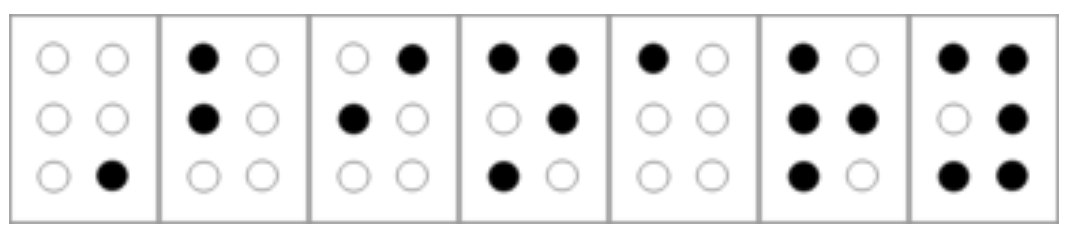
\includegraphics[width=\linewidth, height=1.5in, keepaspectratio]{../figure/braille.png}
\caption{The word ``Binary'' in ``Grade 1'' or ``uncontracted'' Unified
English Braille. This word is encoded using seven symbols since the
first one is a modifier indicating that the first letter is
capitalized.}
\label{braillefig}
\end{marginfigure}

\hypertarget{braille}{}
\begin{example}[The Braille representation] \label[example]{braille}

The \emph{Braille system} is another way to encode letters and other
symbols as binary strings. Specifically, in Braille, every letter is
encoded as a string in \(\{0,1\}^6\), which is written using indented
dots arranged in two columns and three rows, see \cref{braillefig}.
(Some symbols require more than one six-bit string to encode, and so
Braille uses a more general prefix-free encoding.)

The Braille system was invented in 1821 by
\href{https://goo.gl/Y2BkEe}{Louis Braille} when he was just 12 years
old (though he continued working on it and improving it throughout his
life). Braille was a French boy who lost his eyesight at the age of 5 as
the result of an accident.

\end{example}

\hypertarget{Crepresentation}{}
\begin{example}[Representing objects in C (optional)] \label[example]{Crepresentation}

We can use programming languages to probe how our computing environment
represents various values. This is easiest to do in ``unsafe''
programming languages such as \texttt{C} that allow direct access to the
memory.

Using a \href{https://goo.gl/L8oMzn}{simple \texttt{C} program} we have
produced the following representations of various values. One can see
that for integers, multiplying by 2 corresponds to a ``left shift''
inside each byte. In contrast, for floating point numbers, multiplying
by two corresponds to adding one to the exponent part of the
representation. In the architecture we used, a negative number is
represented using the \href{https://goo.gl/wov5fa}{two's complement}
approach. \texttt{C} represents strings in a prefix-free form by
ensuring that a zero byte is at their end.

\begin{code}
int      2    : 00000010 00000000 00000000 00000000
int      4    : 00000100 00000000 00000000 00000000
int      513  : 00000001 00000010 00000000 00000000
long     513  : 00000001 00000010 00000000 00000000 00000000 00000000 00000000 00000000
int      -1   : 11111111 11111111 11111111 11111111
int      -2   : 11111110 11111111 11111111 11111111
string   Hello: 01001000 01100101 01101100 01101100 01101111 00000000
string   abcd : 01100001 01100010 01100011 01100100 00000000
float    33.0 : 00000000 00000000 00000100 01000010
float    66.0 : 00000000 00000000 10000100 01000010
float    132.0: 00000000 00000000 00000100 01000011
double   132.0: 00000000 00000000 00000000 00000000 00000000 10000000 01100000 01000000
\end{code}

\end{example}

\subsection{Representing vectors, matrices,
images}\label{Representing-vectors-matr}

Once we can represent numbers and lists of numbers, then we can also
represent \emph{vectors} (which are just lists of numbers). Similarly,
we can represent lists of lists, and thus, in particular, can represent
\emph{matrices}. To represent an image, we can represent the color at
each pixel by a list of three numbers corresponding to the intensity of
Red, Green and Blue. (We can restrict to three primary colors since
\href{https://en.wikipedia.org/wiki/Tetrachromacy}{most} humans only
have three types of cones in their retinas; we would have needed 16
primary colors to represent colors visible to the
\href{https://goo.gl/t7JBfC}{Mantis Shrimp}.) Thus an image of \(n\)
pixels would be represented by a list of \(n\) such length-three lists.
A video can be represented as a list of images. Of course these
representations are rather wasteful and
\href{https://en.wikipedia.org/wiki/JPEG}{much}
\href{https://goo.gl/Vs8UhU}{more} compact representations are typically
used for images and videos, though this will not be our concern in this
book.

\subsection{Representing graphs}\label{Representing-graphs}

A \emph{graph} on \(n\) vertices can be represented as an \(n\times n\)
\emph{adjacency} matrix whose \((i,j)^{th}\) entry is equal to \(1\) if
the edge \((i,j)\) is present and is equal to \(0\) otherwise. That is,
we can represent an \(n\) vertex directed graph \(G=(V,E)\) as a string
\(A\in \{0,1\}^{n^2}\) such that \(A_{i,j}=1\) iff the edge
\(\overrightarrow{i\;j}\in E\). We can transform an undirected graph to
a directed graph by replacing every edge \(\{i,j\}\) with both edges
\(\overrightarrow{i\; j}\) and \(\overleftarrow{i\;j}\)

Another representation for graphs is the \emph{adjacency list}
representation. That is, we identify the vertex set \(V\) of a graph
with the set \([n]\) where \(n=|V|\), and represent the graph
\(G=(V,E)\) as a list of \(n\) lists, where the \(i\)-th list consists
of the out-neighbors of vertex \(i\). The difference between these
representations can be significant for some applications, though for us
would typically be immaterial.


\begin{marginfigure}
\centering
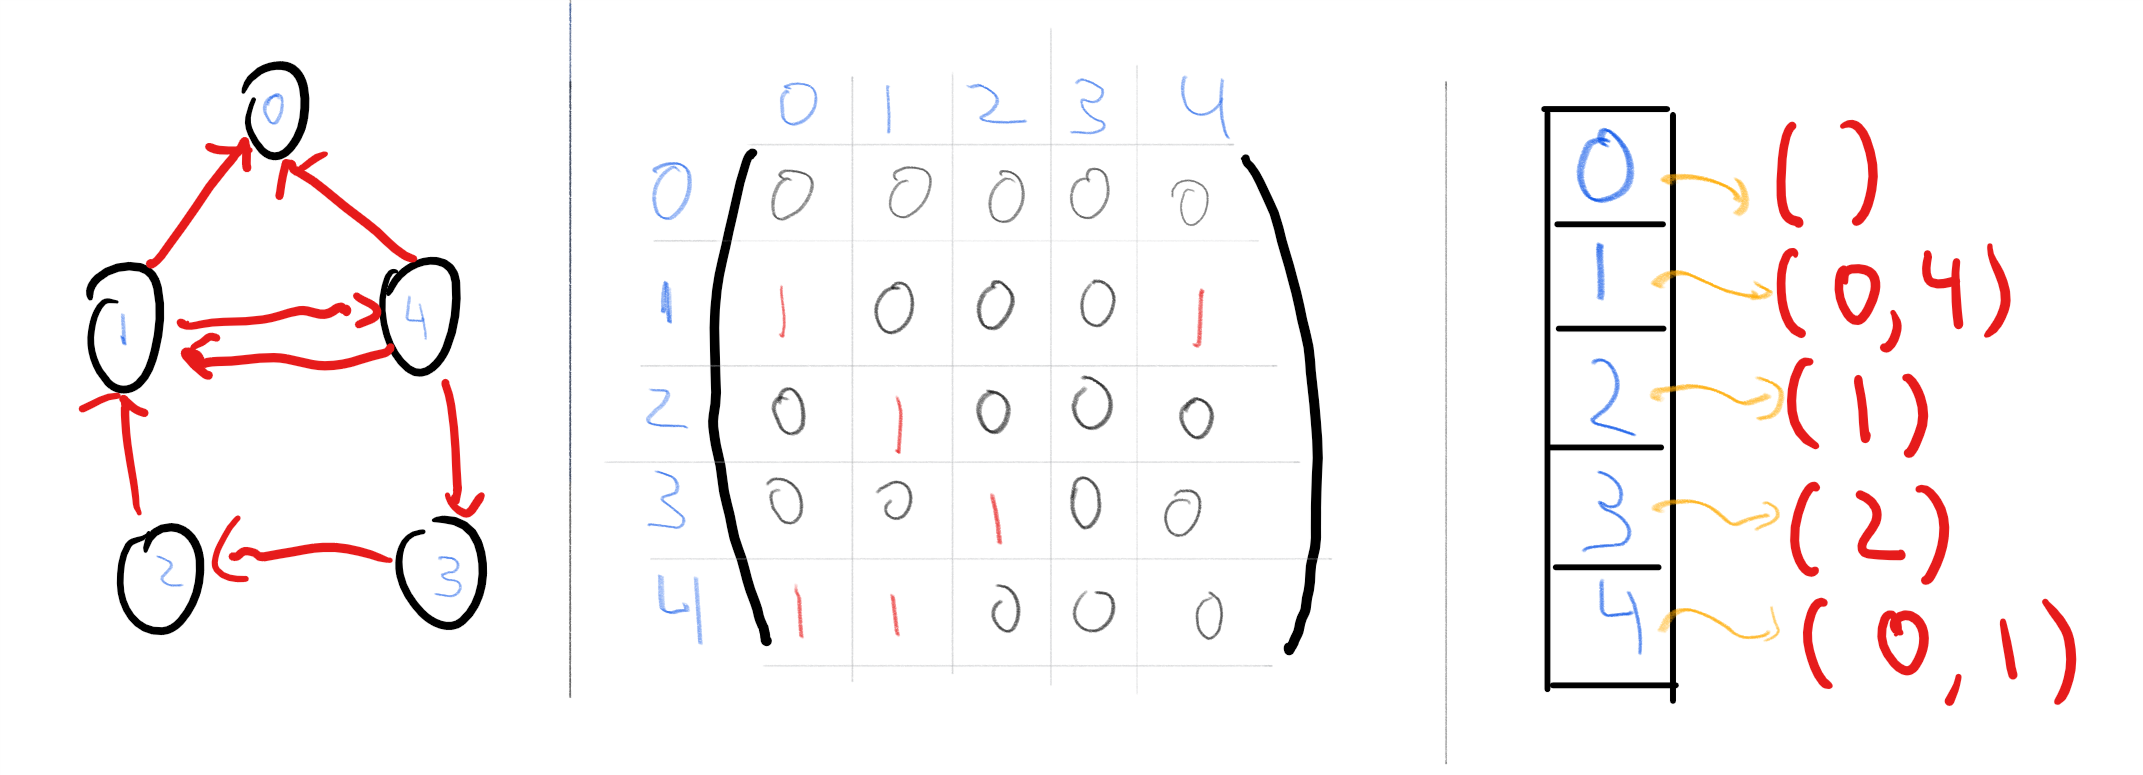
\includegraphics[width=\linewidth, height=1.5in, keepaspectratio]{../figure/representing_graphs.png}
\caption{Representing the graph
\(G=(\{0,1,2,3,4\},\{ (1,0),(4,0),(1,4),(4,1),(2,1),(3,2),(4,3) \})\) in
the adjacency matrix and adjacency list representations.}
\label{representinggraphsfig}
\end{marginfigure}

\subsection{Representing lists and nested
lists}\label{Representing-lists-and-ne}

If we have a way of representing objects from a set \(\mathcal{O}\) as
binary strings, then we can represent lists of these objects by applying
a prefix-free transformation. Moreover, we can use a trick similar to
the above to handle \emph{nested} lists. The idea is that if we have
some representation \(E:\mathcal{O} \rightarrow \{0,1\}^*\), then we can
represent nested lists of items from \(\mathcal{O}\) using strings over
the five element alphabet \(\Sigma = \{\)
\texttt{0},\texttt{1},\texttt{[} , \texttt{]} , \texttt{,} \(\}\). For
example, if \(o_1\) is represented by \texttt{0011}, \(o_2\) is
represented by \texttt{10011}, and \(o_3\) is represented by
\texttt{00111}, then we can represent the nested list
\((o_1,(o_2,o_3))\) as the string \texttt{"[0011,[10011,00111]]"} over
the alphabet \(\Sigma\). By encoding every element of \(\Sigma\) itself
as a three-bit string, we can transform any representation for objects
\(\mathcal{O}\) into a representation that enables representing
(potentially nested) lists of these objects.

\subsection{Notation}\label{Notation}

We will typically identify an object with its representation as a
string. For example, if \(F:\{0,1\}^* \rightarrow \{0,1\}^*\) is some
function that maps strings to strings and \(n\) is an integer, we might
make statements such as ``\(F(n)+1\) is prime'' to mean that if we
represent \(n\) as a string \(x\), then the integer \(m\) represented by
the string \(F(x)\) satisfies that \(m+1\) is prime. (You can see how
this convention of identifying objects with their representation can
save us a lot of cumbersome formalism.) Similarly, if \(x,y\) are some
objects and \(F\) is a function that takes strings as inputs, then by
\(F(x,y)\) we will mean the result of applying \(F\) to the
representation of the ordered pair \((x,y)\). We use the same notation
to invoke functions on \(k\)-tuples of objects for every \(k\).

This convention of identifying an object with its representation as a
string is one that we humans follow all the time. For example, when
people say a statement such as ``\(17\) is a prime number'', what they
really mean is that the integer whose decimal representation is the
string ``\texttt{17}'', is prime.

\begin{quote} \label[quote]{When-we-sayA-is-an-algori}

When we say

\emph{\(A\) is an algorithm that computes the multiplication function on
natural numbers.}

what we really mean is that

\emph{\(A\) is an algorithm that computes the function
\(F:\{0,1\}^* \rightarrow \{0,1\}^*\) such that for every pair
\(a,b \in \N\), if \(x\in \{0,1\}^*\) is a string representing the pair
\((a,b)\) then \(F(x)\) will be a string representing their product
\(a\cdot b\).}

\end{quote}

\section{Defining computational tasks as mathematical
functions}\label{Defining-computational-ta}

Abstractly, a \emph{computational process} is some process that takes an
input which is a string of bits and produces an output which is a string
of bits. This transformation of input to output can be done using a
modern computer, a person following instructions, the evolution of some
natural system, or any other means.

In future chapters, we will turn to mathematically defining
computational processes, but, as we discussed above, at the moment we
focus on \emph{computational tasks}. That is, we focus on the
\textbf{specification} and not the \textbf{implementation}. Again, at an
abstract level, a computational task can specify any relation that the
output needs to have with the input. However, for most of this book, we
will focus on the simplest and most common task of \emph{computing a
function}. Here are some examples:

\begin{itemize}
\item
  Given (a representation of) two integers \(x,y\), compute the product
  \(x\times y\). Using our representation above, this corresponds to
  computing a function from \(\{0,1\}^*\) to \(\{0,1\}^*\). We have seen
  that there is more than one way to solve this computational task, and
  in fact, we still do not know the best algorithm for this problem.
\item
  Given (a representation of) an integer \(z>1\), compute its
  \emph{factorization}; i.e., the list of primes
  \(p_1 \leq \cdots \leq p_k\) such that \(z = p_1\cdots p_k\). This
  again corresponds to computing a function from \(\{0,1\}^*\) to
  \(\{0,1\}^*\). The gaps in our knowledge of the complexity of this
  problem are even larger.
\item
  Given (a representation of) a graph \(G\) and two vertices \(s\) and
  \(t\), compute the length of the shortest path in \(G\) between \(s\)
  and \(t\), or do the same for the \emph{longest} path (with no
  repeated vertices) between \(s\) and \(t\). Both these tasks
  correspond to computing a function from \(\{0,1\}^*\) to
  \(\{0,1\}^*\), though it turns out that there is a vast difference in
  their computational difficulty.
\item
  Given the code of a Python program, determine whether there is an
  input that would force it into an infinite loop. This task corresponds
  to computing a \emph{partial} function from \(\{0,1\}^*\) to
  \(\{0,1\}\) since not every string corresponds to a syntactically
  valid Python program. We will see that we \emph{do} understand the
  computational status of this problem, but the answer is quite
  surprising.
\item
  Given (a representation of) an image \(I\), decide if \(I\) is a photo
  of a cat or a dog. This corresponds to computing some (partial)
  function from \(\{0,1\}^*\) to \(\{0,1\}\).
\end{itemize}

\hypertarget{booleanrem}{}
\begin{remark}[Boolean functions and languages] \label[remark]{booleanrem}

An important special case of computational tasks corresponds to
computing \emph{Boolean} functions, whose output is a single bit
\(\{0,1\}\). Computing such functions corresponds to answering a YES/NO
question, and hence this task is also known as a \emph{decision
problem}. Given any function \(F:\{0,1\}^* \rightarrow \{0,1\}\) and
\(x\in \{0,1\}^*\), the task of computing \(F(x)\) corresponds to the
task of deciding whether or not \(x\in L\) where
\(L = \{ x : F(x)=1 \}\) is known as the \emph{language} that
corresponds to the function \(F\). (The language terminology is due to
historical connections between the theory of computation and formal
linguistics as developed by Noam Chomsky.) Hence many texts refer to
such a computational task as \emph{deciding a language}.

\end{remark}


\begin{marginfigure}
\centering
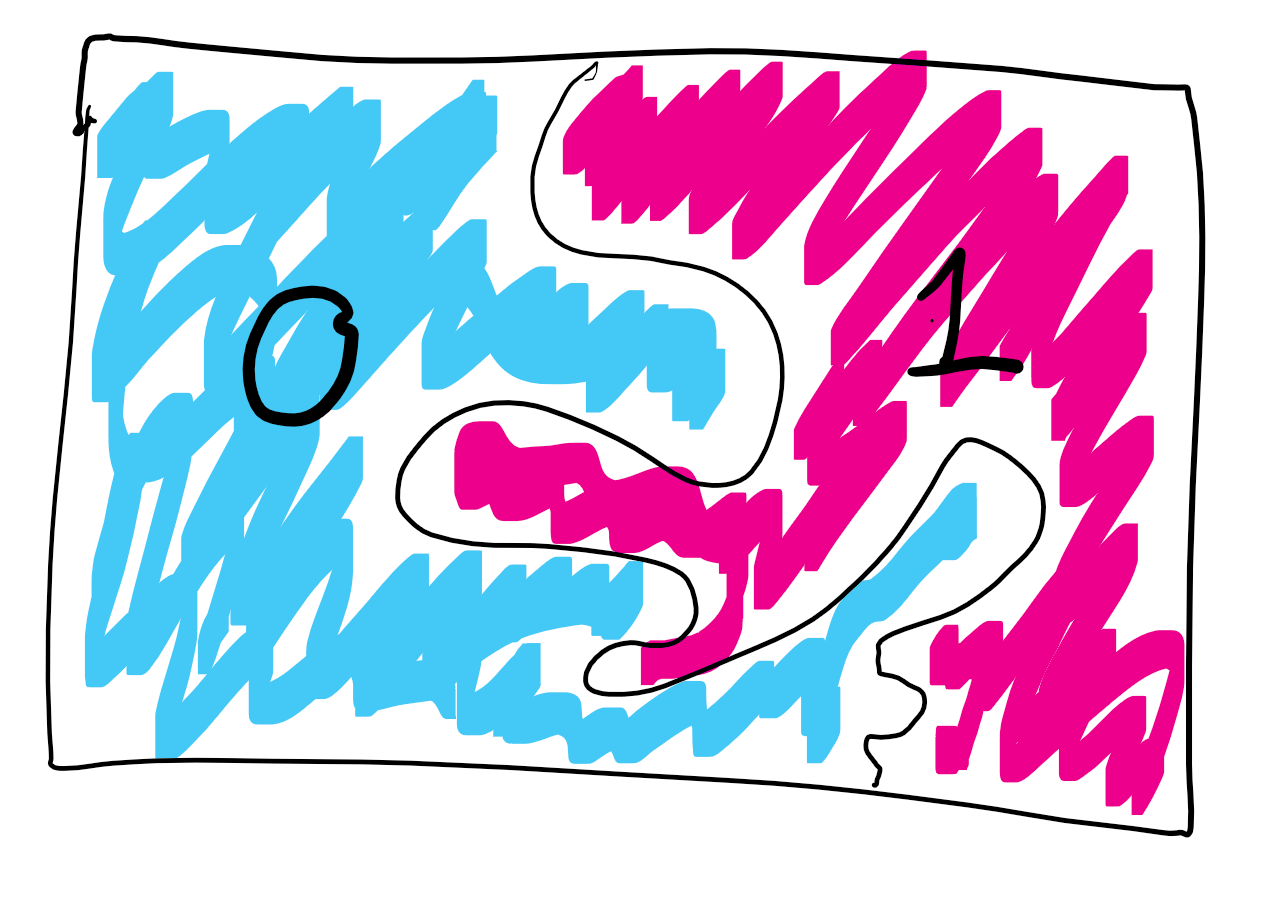
\includegraphics[width=\linewidth, height=1.5in, keepaspectratio]{../figure/booleanfunc.png}
\caption{A subset \(L \subseteq \{0,1\}^*\) can be identified with the
function \(F:\{0,1\}^* \rightarrow \{0,1\}\) such that \(F(x)=1\) if
\(x\in L\) and \(F(x)=0\) if \(x\not\in L\). Functions with a single bit
of output are called \emph{Boolean functions}, while subsets of strings
are called \emph{languages}. The above shows that the two are
essentially the same object, and we can identify the task of deciding
membership in \(L\) (known as \emph{deciding a language} in the
literature) with the task of computing the function \(F\).}
\label{booleanlangfig}
\end{marginfigure}

For every particular function \(F\), there can be several possible
\emph{algorithms} to compute \(F\). We will be interested in questions
such as:

\begin{itemize}
\item
  For a given function \(F\), can it be the case that \emph{there is no
  algorithm} to compute \(F\)?
\item
  If there is an algorithm, what is the best one? Could it be that \(F\)
  is ``effectively uncomputable'' in the sense that every algorithm for
  computing \(F\) requires a prohibitively large amount of resources?
\item
  If we cannot answer this question, can we show equivalence between
  different functions \(F\) and \(F'\) in the sense that either they are
  both easy (i.e., have fast algorithms) or they are both hard?
\item
  Can a function being hard to compute ever be a \emph{good thing}? Can
  we use it for applications in areas such as cryptography?
\end{itemize}

In order to do that, we will need to mathematically define the notion of
an \emph{algorithm}, which is what we will do in \cref{compchap}.

\subsection{Distinguish functions from programs!}\label{secimplvsspec}

You should always watch out for potential confusions between
\textbf{specifications} and \textbf{implementations} or equivalently
between \textbf{mathematical functions} and
\textbf{algorithms/programs}. It does not help that programming
languages (Python included) use the term \emph{``functions''} to denote
(parts of) \emph{programs}. This confusion also stems from thousands of
years of mathematical history, where people typically defined functions
by means of a way to compute them.

For example, consider the multiplication function on natural numbers.
This is the function
\(\ensuremath{\mathit{MULT}}:\N\times \N \rightarrow \N\) that maps a
pair \((x,y)\) of natural numbers to the number \(x \cdot y\). As we
mentioned, it can be implemented in more than one way:

\begin{code}
def mult1(x,y):
    res = 0
    while y>0:
        res += x
        y   -= 1
    return res

def mult2(x,y):
    a = str(x) # represent x as string in decimal notation
    b = str(y) # represent y as string in decimal notation
    res = 0
    for i in range(len(a)):
        for j in range(len(b)):
            res += int(a[len(a)-i])*int(b[len(b)-j])*(10**(i+j))
    return res

print(mult1(12,7))
# 84
print(mult2(12,7))
# 84
\end{code}

Both \texttt{mult1} and \texttt{mult2} produce the same output given the
same pair of natural number inputs. (Though \texttt{mult1} will take far
longer to do so when the numbers become large.) Hence, even though these
are two different \emph{programs}, they compute the same
\emph{mathematical function}. This distinction between a \emph{program}
or \emph{algorithm} \(A\), and the \emph{function} \(F\) that \(A\)
\emph{computes} will be absolutely crucial for us in this course (see
also \cref{functionornotfig}).


\begin{marginfigure}
\centering
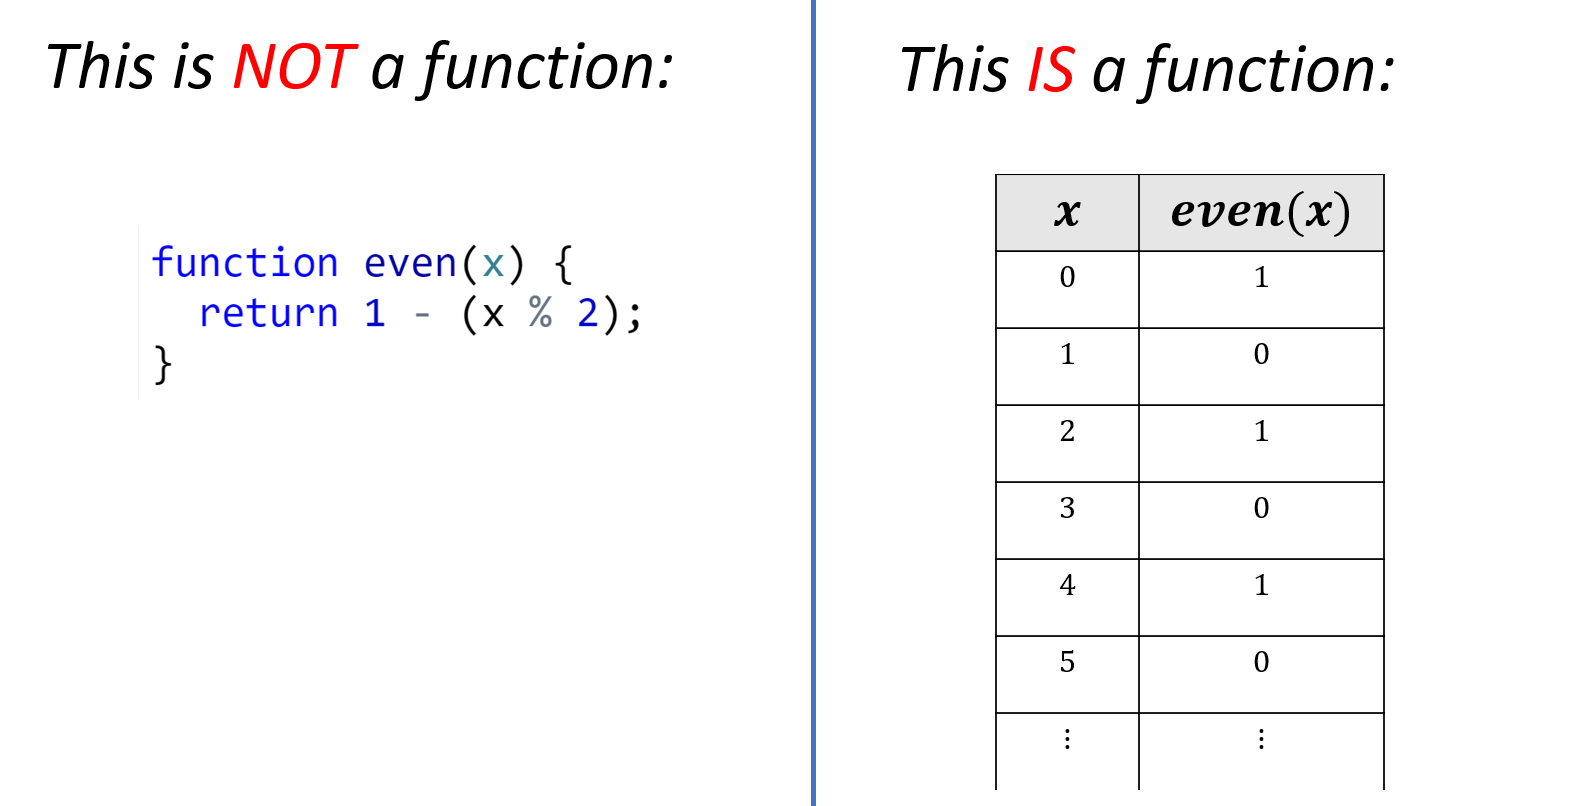
\includegraphics[width=\linewidth, height=1.5in, keepaspectratio]{../figure/functionornot.png}
\caption{A \emph{function} is a mapping of inputs to outputs. A
\emph{program} is a set of instructions on how to obtain an output given
an input. A program \emph{computes} a function, but it is not the same
as a function, popular programming language terminology
notwithstanding.}
\label{functionornotfig}
\end{marginfigure}

\hypertarget{functionprogramidea}{}
\begin{bigidea} \label[bigidea]{functionprogramidea}

A \emph{function} is not the same as a \emph{program}. A program
\emph{computes} a function.

\end{bigidea}

Distinguishing \emph{functions} from \emph{programs} (or other ways for
computing, including \emph{circuits} and \emph{machines}) is a crucial
theme for this course. For this reason, this is often a running theme in
questions that I (and many other instructors) assign in homework and
exams (hint, hint).

\hypertarget{beyonfdunc}{}
\begin{remark}[Computation beyond functions (advanced, optional)] \label[remark]{beyonfdunc}

Functions capture quite a lot of computational tasks, but one can
consider more general settings as well. For starters, we can and will
talk about \emph{partial} functions, that are not defined on all inputs.
When computing a partial function, we only need to worry about the
inputs on which the function is defined. Another way to say it is that
we can design an algorithm for a partial function \(F\) under the
assumption that someone ``promised'' us that all inputs \(x\) would be
such that \(F(x)\) is defined (as otherwise, we do not care about the
result). Hence such tasks are also known as \emph{promise problems}.

Another generalization is to consider \emph{relations} that may have
more than one possible admissible output. For example, consider the task
of finding any solution for a given set of equations. A \emph{relation}
\(R\) maps a string \(x\in \{0,1\}^*\) into a \emph{set of strings}
\(R(x)\) (for example, \(x\) might describe a set of equations, in which
case \(R(x)\) would correspond to the set of all solutions to \(x\)). We
can also identify a relation \(R\) with the set of pairs of strings
\((x,y)\) where \(y\in R(x)\). A computational process solves a relation
if for every \(x\in \{0,1\}^*\), it outputs some string \(y\in R(x)\).

Later in this book, we will consider even more general tasks, including
\emph{interactive} tasks, such as finding a good strategy in a game,
tasks defined using probabilistic notions, and others. However, for much
of this book, we will focus on the task of computing a function, and
often even a \emph{Boolean} function, that has only a single bit of
output. It turns out that a great deal of the theory of computation can
be studied in the context of this task, and the insights learned are
applicable in the more general settings.

\end{remark}

\begin{recap} \label[recap]{We-can-represent-objects-}

\begin{itemize}
\tightlist
\item
  We can represent objects we want to compute on using binary strings.
\item
  A representation scheme for a set of objects \(\mathcal{O}\) is a
  one-to-one map from \(\mathcal{O}\) to \(\{0,1\}^*\).
\item
  We can use prefix-free encoding to ``boost'' a representation for a
  set \(\mathcal{O}\) into representations of lists of elements in
  \(\mathcal{O}\).
\item
  A basic computational task is the task of \emph{computing a function}
  \(F:\{0,1\}^* \rightarrow \{0,1\}^*\). This task encompasses not just
  arithmetical computations such as multiplication, factoring, etc. but
  a great many other tasks arising in areas as diverse as scientific
  computing, artificial intelligence, image processing, data mining and
  many many more.
\item
  We will study the question of finding (or at least giving bounds on)
  what the \emph{best} algorithm for computing \(F\) for various
  interesting functions \(F\) is.
\end{itemize}

\end{recap}

\section{Exercises}\label{Exercises}

\begin{exercise} \label[exercise]{Which-one-of-these-object}

Which one of these objects can be represented by a binary string?

\begin{enumerate}
\def\labelenumi{\alph{enumi}.}
\item
  An integer \(x\)
\item
  An undirected graph \(G\).
\item
  A directed graph \(H\)
\item
  All of the above.
\end{enumerate}

\end{exercise}

\hypertarget{binaryrepex}{}
\begin{exercise}[Binary representation] \label[exercise]{binaryrepex}

\begin{enumerate}
\def\labelenumi{\alph{enumi}.}
\item
  Prove that the function \(NtS:\N \rightarrow \{0,1\}^*\) of the binary
  representation defined in \eqref{ntseq} satisfies that for every
  \(n\in \N\), if \(x = NtS(n)\) then
  \(|x| =1+\max(0,\floor{\log_2 n})\) and
  \(x_i = \floor{x/2^{\floor{\log_2 n}-i}} \mod 2\).
\item
  Prove that \(NtS\) is a one to one function by coming up with a
  function \(StN:\{0,1\}^* \rightarrow \N\) such that \(StN(NtS(n))=n\)
  for every \(n\in \N\).
\end{enumerate}

\end{exercise}

\hypertarget{compactrepletters}{}
\begin{exercise}[More compact than ASCII representation] \label[exercise]{compactrepletters}

The ASCII encoding can be used to encode a string of \(n\) English
letters as a \(7n\) bit binary string, but in this exercise, we ask
about finding a more compact representation for strings of English
lowercase letters.

\begin{enumerate}
\def\labelenumi{\arabic{enumi}.}
\item
  Prove that there exists a representation scheme \((E,D)\) for strings
  over the 26-letter alphabet \(\{ a, b,c,\ldots,z \}\) as binary
  strings such that for every \(n>0\) and length-\(n\) string
  \(x \in \{ a,b,\ldots,z \}^n\), the representation \(E(x)\) is a
  binary string of length at most \(4.8n+1000\). In other words, prove
  that for every \(n\), there exists a one-to-one function
  \(E:\{a,b,\ldots, z\}^n \rightarrow \{0,1\}^{\lfloor 4.8n +1000 \rfloor}\).
\item
  Prove that there exists \emph{no} representation scheme for strings
  over the alphabet \(\{ a, b,\ldots,z \}\) as binary strings such that
  for every length-\(n\) string \(x \in \{ a,b,\ldots, z\}^n\), the
  representation \(E(x)\) is a binary string of length
  \(\lfloor 4.6n+1000 \rfloor\). In other words, prove that there exists
  some \(n>0\) such that there is no one-to-one function
  \(E:\{a,b,\ldots,z \}^n \rightarrow \{0,1\}^{\lfloor 4.6n + 1000 \rfloor}\)
\item
  Python's \texttt{bz2.compress} function is a mapping from strings to
  strings, which uses the \emph{lossless} (and hence \emph{one to one})
  \href{https://en.wikipedia.org/wiki/Bzip2}{bzip2} algorithm for
  compression. After converting to lowercase, and truncating spaces and
  numbers, the text of Tolstoy's ``War and Peace'' contains
  \(n=2,517,262\). Yet, if we run \texttt{bz2.compress} on the string of
  the text of ``War and Peace'' we get a string of length
  \(k=6,274,768\) bits, which is only \(2.49n\) (and in particular much
  smaller than \(4.6n\)). Explain why this does not contradict your
  answer to the previous question.
\item
  Interestingly, if we try to apply \texttt{bz2.compress} on a
  \emph{random} string, we get much worse performance. In my
  experiments, I got a ratio of about \(4.78\) between the number of
  bits in the output and the number of characters in the input. However,
  one could imagine that one could do better and that there exists a
  company called ``Pied Piper'' with an algorithm that can losslessly
  compress a string of \(n\) random lowercase letters to fewer than
  \(4.6n\) bits.\footnote{Actually that particular fictional company
    uses a metric that focuses more on compression \emph{speed} then
    \emph{ratio}, see
    \href{https://blogs.dropbox.com/tech/2016/06/lossless-compression-with-brotli/}{here}
    and \href{https://www.jefftk.com/p/weissman-scores-useful}{here}.}
  Show that this is not the case by proving that for \emph{every}
  \(n>100\) and one to one function
  \(Encode:\{a,\ldots,z\}^{n} \rightarrow \{0,1\}^*\), if we let \(Z\)
  be the random variable \(|Encode(x)|\) (i.e., the length of
  \(Encode(x)\)) for \(x\) chosen uniformly at random from the set
  \(\{a,\ldots,z\}^n\), then the expected value of \(Z\) is at least
  \(4.6n\).
\end{enumerate}

\end{exercise}

\hypertarget{representinggraphsex}{}
\begin{exercise}[Representing graphs: upper bound] \label[exercise]{representinggraphsex}

Show that there is a string representation of directed graphs with
vertex set \([n]\) and degree at most \(10\) that uses at most
\(1000 n\log n\) bits. More formally, show the following: Suppose we
define for every \(n\in\mathbb{N}\), the set \(G_n\) as the set
containing all directed graphs (with no self loops) over the vertex set
\([n]\) where every vertex has degree at most \(10\). Then, prove that
for every sufficiently large \(n\), there exists a one-to-one function
\(E:G_n \rightarrow \{0,1\}^{\lfloor 1000 n \log n \rfloor}\).

\end{exercise}

\hypertarget{represgraphlbex}{}
\begin{exercise}[Representing graphs: lower bound] \label[exercise]{represgraphlbex}

\begin{enumerate}
\def\labelenumi{\arabic{enumi}.}
\item
  Define \(S_n\) to be the set of one-to-one and onto functions mapping
  \([n]\) to \([n]\). Prove that there is a one-to-one mapping from
  \(S_n\) to \(G_{2n}\), where \(G_{2n}\) is the set defined in
  \cref{representinggraphsex} above.
\item
  In this question you will show that one cannot improve the
  representation of \cref{representinggraphsex} to length
  \(o(n \log n)\). Specifically, prove for every sufficiently large
  \(n\in \mathbb{N}\) there is \emph{no} one-to-one function
  \(E:G_n \rightarrow \{0,1\}^{\lfloor 0.001 n \log n \rfloor +1000}\).
\end{enumerate}

\end{exercise}

\hypertarget{multrepres}{}
\begin{exercise}[Multiplying in different representation] \label[exercise]{multrepres}

Recall that the grade-school algorithm for multiplying two numbers
requires \(O(n^2)\) operations. Suppose that instead of using decimal
representation, we use one of the following representations \(R(x)\) to
represent a number \(x\) between \(0\) and \(10^n-1\). For which one of
these representations you can still multiply the numbers in \(O(n^2)\)
operations?

\begin{enumerate}
\def\labelenumi{\alph{enumi}.}
\item
  The standard binary representation: \(B(x)=(x_0,\ldots,x_{k})\) where
  \(x = \sum_{i=0}^{k} x_i 2^i\) and \(k\) is the largest number s.t.
  \(x \geq 2^k\).
\item
  The reverse binary representation: \(B(x) = (x_{k},\ldots,x_0)\) where
  \(x_i\) is defined as above for \(i=0,\ldots,k-1\).\\
\item
  Binary coded decimal representation: \(B(x)=(y_0,\ldots,y_{n-1})\)
  where \(y_i \in \{0,1\}^4\) represents the \(i^{th}\) decimal digit of
  \(x\) mapping \(0\) to \(0000\), \(1\) to \(0001\), \(2\) to \(0010\),
  etc. (i.e.~\(9\) maps to \(1001\))
\item
  All of the above.
\end{enumerate}

\end{exercise}

\begin{exercise} \label[exercise]{Suppose-that-RN-rightarro}

Suppose that \(R:\N \rightarrow \{0,1\}^*\) corresponds to representing
a number \(x\) as a string of \(x\) \(1\)'s, (e.g., \(R(4)=1111\),
\(R(7)=1111111\), etc.). If \(x,y\) are numbers between \(0\) and
\(10^n -1\), can we still multiply \(x\) and \(y\) using \(O(n^2)\)
operations if we are given them in the representation \(R(\cdot)\)?

\end{exercise}

\begin{exercise} \label[exercise]{Recall-that-if-F-is-a-one}

Recall that if \(F\) is a one-to-one and onto function mapping elements
of a finite set \(U\) into a finite set \(V\) then the sizes of \(U\)
and \(V\) are the same. Let \(B:\N\rightarrow\{0,1\}^*\) be the function
such that for every \(x\in\N\), \(B(x)\) is the binary representation of
\(x\).

\begin{enumerate}
\def\labelenumi{\arabic{enumi}.}
\item
  Prove that \(x < 2^k\) if and only if \(|B(x)| \leq k\).
\item
  Use 1. to compute the size of the set
  \(\{ y \in \{0,1\}^* : |y| \leq k \}\) where \(|y|\) denotes the
  length of the string \(y\).
\item
  Use 1. and 2. to prove that \(2^k-1 = 1 + 2 + 4+ \cdots + 2^{k-1}\).
\end{enumerate}

\end{exercise}

\hypertarget{prefix-free-tuples-ex}{}
\begin{exercise}[Prefix-free encoding of tuples] \label[exercise]{prefix-free-tuples-ex}

Suppose that \(F:\N\rightarrow\{0,1\}^*\) is a one-to-one function that
is \emph{prefix-free} in the sense that there is no \(a\neq b\) s.t.
\(F(a)\) is a prefix of \(F(b)\).

\begin{enumerate}
\def\labelenumi{\alph{enumi}.}
\item
  Prove that \(F_2:\N\times \N \rightarrow \{0,1\}^*\), defined as
  \(F_2(a,b) = F(a)F(b)\) (i.e., the concatenation of \(F(a)\) and
  \(F(b)\)) is a one-to-one function.
\item
  Prove that \(F_*:\N^*\rightarrow\{0,1\}^*\) defined as
  \(F_*(a_1,\ldots,a_k) = F(a_1)\cdots F(a_k)\) is a one-to-one
  function, where \(\N^*\) denotes the set of all finite-length lists of
  natural numbers.
\end{enumerate}

\end{exercise}

\hypertarget{prefix-free-ex}{}
\begin{exercise}[More efficient prefix-free transformation] \label[exercise]{prefix-free-ex}

Suppose that \(F:O\rightarrow\{0,1\}^*\) is some (not necessarily
prefix-free) representation of the objects in the set \(O\), and
\(G:\N\rightarrow\{0,1\}^*\) is a prefix-free representation of the
natural numbers. Define \(F'(o)=G(|F(o)|)F(o)\) (i.e., the concatenation
of the representation of the length \(F(o)\) and \(F(o)\)).

\begin{enumerate}
\def\labelenumi{\alph{enumi}.}
\item
  Prove that \(F'\) is a prefix-free representation of \(O\).
\item
  Show that we can transform any representation to a prefix-free one by
  a modification that takes a \(k\) bit string into a string of length
  at most \(k+O(\log k)\).
\item
  Show that we can transform any representation to a prefix-free one by
  a modification that takes a \(k\) bit string into a string of length
  at most \(k+ \log k + O(\log\log k)\).\footnote{Hint: Think
    recursively how to represent the length of the string.}
\end{enumerate}

\end{exercise}

\hypertarget{prefix-free-lb}{}
\begin{exercise}[Kraft's Inequality] \label[exercise]{prefix-free-lb}

Suppose that \(S \subseteq \{0,1\}^n\) is some finite prefix-free set.

\begin{enumerate}
\def\labelenumi{\alph{enumi}.}
\item
  For every \(k \leq n\) and length-\(k\) string \(x\in S\), let
  \(L(x) \subseteq \{0,1\}^n\) denote all the length-\(n\) strings whose
  first \(k\) bits are \(x_0,\ldots,x_{k-1}\). Prove that \textbf{(1)}
  \(|L(x)|=2^{n-|x|}\) and \textbf{(2)} If \(x \neq x'\) then \(L(x)\)
  is disjoint from \(L(x')\).
\item
  Prove that \(\sum_{x\in S}2^{-|x|} \leq 1\).
\item
  Prove that there is no prefix-free encoding of strings with less than
  logarithmic overhead. That is, prove that there is no function
  \(\ensuremath{\mathit{PF}}:\{0,1\}^* \rightarrow \{0,1\}^*\) s.t.
  \(|\ensuremath{\mathit{PF}}(x)| \leq |x|+0.9\log |x|\) for every
  \(x\in \{0,1\}^*\) and such that the set
  \(\{ \ensuremath{\mathit{PF}}(x) : x\in \{0,1\}^* \}\) is prefix-free.
  The factor \(0.9\) is arbitrary; all that matters is that it is less
  than \(1\).
\end{enumerate}

\end{exercise}

\hypertarget{onetoonecompex}{}
\begin{exercise}[Composition of one-to-one functions] \label[exercise]{onetoonecompex}

Prove that for every two one-to-one functions \(F:S \rightarrow T\) and
\(G:T \rightarrow U\), the function \(H:S \rightarrow U\) defined as
\(H(x)=G(F(x))\) is one to one.

\end{exercise}

\hypertarget{naturalsstringsmapex}{}
\begin{exercise}[Natural numbers and strings] \label[exercise]{naturalsstringsmapex}

\begin{enumerate}
\def\labelenumi{\arabic{enumi}.}
\item
  We have shown that the natural numbers can be represented as strings.
  Prove that the other direction holds as well: that there is a
  one-to-one map \(StN:\{0,1\}^* \rightarrow \N\). (\(StN\) stands for
  ``strings to numbers.'')
\item
  Recall that Cantor proved that there is no one-to-one map
  \(RtN:\R \rightarrow \N\). Show that Cantor's result implies
  \cref{cantorthm}.
\end{enumerate}

\end{exercise}

\hypertarget{listsinttonumex}{}
\begin{exercise}[Map lists of integers to a number] \label[exercise]{listsinttonumex}

Recall that for every set \(S\), the set \(S^*\) is defined as the set
of all finite sequences of members of \(S\) (i.e.,
\(S^* = \{ (x_0,\ldots,x_{n-1}) \;|\; n\in\mathbb{N} \;,\; \forall_{i\in [n]} x_i \in S \}\)
). Prove that there is a one-one-map from \(\mathbb{Z}^*\) to
\(\mathbb{N}\) where \(\mathbb{Z}\) is the set of
\(\{ \ldots, -3 , -2 , -1,0,+1,+2,+3,\ldots \}\) of all integers.

\end{exercise}

\section{Bibliographical notes}\label{bibnotesrepres}

The study of representing data as strings, including issues such as
\emph{compression} and \emph{error corrections} falls under the purview
of \emph{information theory}, as covered in the classic textbook of
Cover and Thomas \cite{CoverThomas06}. Representations are also studied
in the field of \emph{data structures design}, as covered in texts such
as \cite{CLRS}.

The question of whether to represent integers with the most significant
digit first or last is known as
\href{https://betterexplained.com/articles/understanding-big-and-little-endian-byte-order/}{Big
Endian vs.~Little Endian} representation. This terminology comes from
Cohen's \cite{cohen1981holy} entertaining and informative paper about
the conflict between adherents of both schools which he compared to the
warring tribes in Jonathan Swift's \emph{``Gulliver's Travels''}. The
two's complement representation of signed integers was suggested in von
Neumann's classic report \cite{vonNeumann45} that detailed the design
approaches for a stored-program computer, though similar representations
have been used even earlier in abacus and other mechanical computation
devices.

The idea that we should separate the \emph{definition} or
\emph{specification} of a function from its \emph{implementation} or
\emph{computation} might seem ``obvious,'' but it took quite a lot of
time for mathematicians to arrive at this viewpoint. Historically, a
function \(F\) was identified by rules or formulas showing how to derive
the output from the input. As we discuss in greater depth in
\cref{chapcomputable}, in the 1800s this somewhat informal notion of a
function started ``breaking at the seams,'' and eventually
mathematicians arrived at the more rigorous definition of a function as
an arbitrary assignment of input to outputs. While many functions may be
described (or computed) by one or more formulas, today we do not
consider that to be an essential property of functions, and also allow
functions that do not correspond to any ``nice'' formula.

We have mentioned that all representations of the real numbers are
inherently \emph{approximate}. Thus an important endeavor is to
understand what guarantees we can offer on the approximation quality of
the output of an algorithm, as a function of the approximation quality
of the inputs. This question is known as the question of determining the
\href{https://en.wikipedia.org/wiki/Numerical_stability}{numerical
stability} of given equations. The
\href{https://floating-point-gui.de/}{Floating Points Guide website}
contains an extensive description of the floating point representation,
as well the many ways in which it could subtly fail, see also the
website \href{http://0.30000000000000004.com/}{0.30000000000000004.com}.

Dauben \cite{Dauben90cantor} gives a biography of Cantor with emphasis
on the development of his mathematical ideas. \cite{halmos1960naive} is
a classic textbook on set theory, including also Cantor's theorem.
Cantor's Theorem is also covered in many texts on discrete mathematics,
including \cite{LehmanLeightonMeyer , LewisZax19 }.

The adjacency matrix representation of graphs is not merely a convenient
way to map a graph into a binary string, but it turns out that many
natural notions and operations on matrices are useful for graphs as
well. (For example, Google's PageRank algorithm relies on this
viewpoint.) The notes of
\href{http://www.cs.yale.edu/homes/spielman/561/}{Spielman's course} are
an excellent source for this area, known as \emph{spectral graph
theory}. We will return to this view much later in this book when we
talk about \emph{random walks}.
